% hoot.tex

% Author: Dustin Bachrach, Christopher Nunu, Dan Wallach, Matt Wright

% Revisions:  28 March 2011

\documentclass{sig-alternate-arxiv}
%\documentclass{acm_proc_article-sp}

\usepackage{amsmath}
\usepackage{times}
\usepackage{mathptm}
\usepackage[scaled=0.87]{helvet} % better visual match w/ Times
\usepackage{graphicx}
\usepackage{balance}
\usepackage{soul}
\usepackage{color}
\usepackage{xspace}
\usepackage{url} \urlstyle{sf}
%\usepackage[draft,inline,nomargin]{fixme}
\usepackage[final,inline,nomargin]{fixme}
\usepackage{clrscode} % fancy coding FTW

\newcommand{\hlfixme}[1]{\fixme{\hl{#1}}}
\newcommand{\hlfxnote}[1]{\fxnote{\hl{#1}}}
\newcommand{\reminder}[1]{[[[ \marginpar{\mbox{$<==$}} {\bf #1} ]]]}
\newcommand{\tasks}[1]{\noindent \textsc{Tasks:} {\it #1}}

\newcommand{\hoot}{{\tt \#h00t}\xspace}
%\newcommand{\hoot}{HooT\xspace}
\newcommand{\msg}{hoot\xspace}
\newcommand{\msgs}{hoots\xspace}

%\newcommand{\paragraph}{\noindent {\bf #1}}
\newcommand{\paragraphX}[1]{\vskip 4pt \noindent \textbf{#1} \hskip .05in}

\graphicspath{{./graphs/}}

\def\sharedaffiliation{%
\end{tabular}
\begin{tabular}{c}}

\begin{document}

\numberofauthors{1} 
\author{
Dustin Bachrach$^{\dag}$, Christopher Nunu$^{\dag}$, Dan S. Wallach$^{\dag}$, Matthew Wright$^{\S}$\\\\
\begin{tabular}{ccc}
\affaddr{$^{\dag}$Dept. of Computer Science} & \hspace{1.2cm} & \affaddr{$^{\S}$Dept. of Computer Science and Engineering}\\
 \affaddr{Rice University} & & \affaddr{University of Texas at Arlington}\\
\affaddr{Houston, Texas, USA} & & \affaddr{Arlington, Texas, USA}  \\
\email{\{ahdustin,canunu\}@gmail.com} & & \email{mwright@cse.uta.edu}\\
\email{dwallach@cs.rice.edu} & &\\
\end{tabular}\\ \\
}

%\numberofauthors{4}
%\author{
%\alignauthor Dustin Bachrach
%\alignauthor Christopher Nunu
%%	\email{canunu@gmail.com}	
%%	\email{dwallach@rice.edu}\\
%\sharedaffiliation
%\hspace{2 cm} \affaddr{Department of Computer Science} \hspace{2 cm} \\
%\hspace{2 cm} \affaddr{Rice University} \hspace{2 cm} \\
%\hspace{2 cm} \affaddr{Houston, Texas} \hspace{2 cm} \\
%\hspace{2 cm} \email{\{ahdustin,canunu\}@gmail.com} \hspace{2 cm} \\	
%\hspace{2 cm}
%\and\\
%\alignauthor Dan Wallach\\
%	\affaddr{Department of Computer Science}\\
%	\affaddr{Rice University}\\
%	\affaddr{Houston, Texas}\\
%	\email{dwallach@rice.edu}\\	
%\alignauthor Matthew Wright\\
%	\affaddr{Department of Computer Science and Engineering}\\
%	\affaddr{University of Texas at Arlington}\\
%	\affaddr{Arlington, Texas}\\
%	\email{mwright@cse.uta.edu}
%}



\title{{\huge \hoot}: Censorship Resistant Microblogging}
%\date{May 6th, 2011}

\maketitle

%\begin{abstract}

%This paper presents the design and engineering of a system called
%HooT. 
Microblogging services such as Twitter are an increasingly important way
to communicate, both for individuals and for groups through the use of
hashtags that denote topics of conversation. However, groups can be
easily blocked from communicating through blocking of posts with the
given hashtags. We propose HooT, a system for censorship-resistant
microblogging. HooT presents an interface that is much like Twitter,
except that hashtags are replaced with very short hashes (e.g. 24 bits)
of the group identifier. Naturally, with such short hashes, hashtags
from different groups may collide and HooT users will actually seek to
create collisions. By encrypting all posts with keys derived from the
group identifiers, Hoot client software can filter out other groups'
posts while making such filtering difficult for the adversary. In
essence, by leveraging collisions, groups can tunnel their posts in
other groups' posts. A censor could not block a given group without also
blocking the other groups with colliding hashtags.
%
%HooT presents an interface that feels much like Twitter, except
%hashtags, which are normally used to denote conversation topics, are
%overloaded with cryptographic semantics; hashtags become cryptographic
%keys.  A HooT can then tunnel through other microblogging services,
%without observers able to read the message unless they know the original
%hashtag or tags that were used when the HooT was created.
%
We evaluate the feasibility of HooT through traces collected from
Twitter, showing that a single modern computer has enough computational
throughput to encrypt every tweet sent through Twitter in real time. We
also use these traces to analyze the bandwidth and anonymity tradeoffs
that would come with different variations on how group identifiers are
encoded and hashtags are selected to purposefully collide with one
another.
%
%Ultimately, censorship resistance and receiver anonymity comes from
%these collisions. A user subscribing to a high-volume innocuous hashtag
%would be indistinguishable from a user subscribing to a low-volume
%subversive hashtag.

\end{abstract}

\begin{abstract}

%This paper presents the design and engineering of a system called
%HooT. 
Microblogging services such as Twitter are an increasingly important way
to communicate, both for individuals and for groups through the use of
hashtags that denote topics of conversation. However, groups can be
easily blocked from communicating through blocking of posts with the
	given hashtags. We propose \hoot, a system for censorship resistant
microblogging. \hoot presents an interface that is much like Twitter,
except that hashtags are replaced with very short hashes (e.g., 24 bits)
of the group identifier. Naturally, with such short hashes, hashtags
from different groups may collide and \hoot users will actually seek to
create collisions. By encrypting all posts with keys derived from the
group identifiers, \hoot client software can filter out other groups'
posts while making such filtering difficult for the adversary. In
essence, by leveraging collisions, groups can tunnel their posts in
other groups' posts. A censor could not block a given group without also
blocking the other groups with colliding hashtags.
%
%HooT presents an interface that feels much like Twitter, except
%hashtags, which are normally used to denote conversation topics, are
%overloaded with cryptographic semantics; hashtags become cryptographic
%keys.  A HooT can then tunnel through other microblogging services,
%without observers able to read the message unless they know the original
%hashtag or tags that were used when the HooT was created.
%
We evaluate the feasibility of \hoot through traces collected from
Twitter, showing that a single modern computer has enough computational
throughput to encrypt every tweet sent through Twitter in real time. We
also use these traces to analyze the bandwidth and anonymity tradeoffs
that would come with different variations on how group identifiers are
encoded and hashtags are selected to purposefully collide with one
another.
%
%Ultimately, censorship resistance and receiver anonymity comes from
%these collisions. A user subscribing to a high-volume innocuous hashtag
%would be indistinguishable from a user subscribing to a low-volume
%subversive hashtag.

\end{abstract}

%\section{Introduction}

Recent events in Egypt, Tunisia, and many other countries have shown that social networking sites (Facebook, Twitter, and presumably others) played a non-trivial role in helping people organize themselves, plan protests, and distribute videos and other news to the outside world. Egypt was notable in that they eventually cut themselves off from the entire Internet, in a belated and ultimately ineffectual attempt to turn the tide. While it's difficult to draw overarching conclusions about the centrality of social networking versus more traditional means of communication in these important world events, it is clear that social media played a non-trivial role. Many other countries' leaders may well be worried of copycat revolutionaries. Other such countries may well try to censor or otherwise tamper with their citizens' use of social networking. To pick a current example: Syria appears to be attempting
a nationwide man-in-the-middle attack against Facebook~\cite{syria-facebook}. 

As a first step toward improving social network systems for such environments, we wish to design a system to enable the use of strong cryptographic primitives, overlaid on existing microblogging services like Twitter. We wish to enable secure group communication without requiring prearranged public key hierarchies or other forms of key exchange. We wish to provide some measure of anonymity, by blurring the binding between the sender and recipients of any given message, using existing innocuous messages as a form of cover traffic, providing some measure of deniability, at least for recipients of messages.

In particular, our work aims to present an interface where most users never see or concern themselves with cryptographic keys. Instead, one of our key insights is that we can overload Twitter's ``hashtag'' mechanism as a way of deriving cryptographic key material. Before we can sort out exactly how that should work, it's important to first understand how hashtags are used in the wild.

Hashtags are widely used in the Twitter universe to label topics which others will then subscribe to and follow. For example, most Usenix conferences adopt the tag {\tt \#usenix}, allowing attendees to discuss the conference with one another in real time. Political protests might end up using several different tags (e.g., Egyptian discussions happen under {\tt \#tahrir}, {\tt \#jan25}, {\tt \#25jan}, and {\tt \#egypt}, among others). Hashtags searches are generally case-insensitive.

Some tags have staggering volumes of messages. To pick a notable example, pop singer Justin Bieber asked his roughly 9 million followers to discuss his movie, {\em Never Say Never} using the hashtag {\tt \#nsn3d}. At its peak, roughly 1\% of Twitter's traffic mentioned this tag\footnote{Statistics via Trendistic, Topsy, and HashTracking.}. Since the movie's release in February 2011, there have been roughly 164 thousand tweets using {\tt \#nsn3d}, an average of 1.6 per minute with significantly higher peaks. 500 recent tweets on this hashtag generated 346 thousand impressions, reaching an audience of 212 thousand followers within a 24 hour period (measured in mid-April 2011). 

Of course, not all tags are as popular. We will show later, in Section~\ref{sec:experiments}, that hashtag usage follows a power-law distribution; a small number of hashtags are incredibly widely used and large numbers of tags are used very rarely or only once. We would like to design a system that can leverage these communications to create cover traffic for other, more sensitive messages, but without simply reusing the popular hashtag for other content. This will require converting hashtags into cryptographic keys and arranging for them to collide in some fashion, such that a query for {\tt \#nsn3d} and a query for a more sensitive tag are indistinguishable to an observer, thus providing some measure of deniability to group subscribers (``Protests? I'm just a fan of Justin Bieber!''). We also need to give some amount of control to the organizers of the sensitive communications, allowing them to select any popular hashtag with which they might prefer to collide.

Ultimately, we see two main paths to designing our system. One option would be to send encrypted messages that include the real {\tt \#nsn3d} tag, perhaps engineering some sort of steganographic process that tries to hide the plaintext within messages that are statistically similar to other posts from Bieber's fan, but it seems inappropriate to produce false messages like this. The other possibility is to imagine that {\em all} Twitter messages are encrypted in a uniform way, where knowing the plaintext of the hashtags would enable the decryption of a message. (It's easy to see a proxy server, of some sort, providing an ``encrypted'' interface to Twitter in this fashion; more on that in \hlfixme{TODO} Section~\ref{sec:whatever-else}.) This is the design we chose to pursue. In this setup, we can encrypt and MAC every message with a random session key, which can be decrypted if the user knows the proper hashtag. ``Encrypted'' hashtags can also be generated by hashing the plaintext hashtags and truncating those hashes.  (We address this unwieldy vocabulary when we present our design in Section~\ref{sec:design}.) Consequently, two different plaintext hashtags can collide with each other with a probability related to the number of bits in the truncated hash.

\if 0
% decided not to use this, and instead convert "threat model" into "design goals"
To make a system like this ``real'', we must:
\begin{itemize}
\item Ensure that real Twitter messages use enough hashtags that, when reflected through our system, provide a significant amount of cover traffic in which to hide other messages.
\item Ensure that hashtags, when used directly as secrets, can be long enough to defeat computational brute force searches, yet be short enough to be memorized and passed along through spoken gossip.
\item Ensure that followers of secret hashtags have a defensible cover story (e.g., ``I'm just a big fan of Justin Bieber!'').
\item Ensure that those who post with secret hashtags can protect themselves from discovery.
\item Ensure that censorship systems, should they not know the secret hashtags, cannot distinguish those messages from other perfectly legitimate messages. We want to ensure that the only surefire way to filter secret messages is to disable the entire social network.
\item Be backward compatible, to the extent possible, with the real Twitter.
\item Minimize the extent to which we need to leverage external anonymity/censorship-resistance systems.
\end{itemize}
\fi

% Our work aims to offer modest improvements to the ability for groups of people to carry out conversations, via social media, 
% 
% \hl{
% - Problem: Twitter like semantics w/ encrypted messages
% 	- Follow a Hash tag
% 	- Take hash tag and create something with crypto strength
% 	- Something derived from tags you can search on
% 	- But also deliberate collisions (cover traffic)
% 	
% - Like to have thing that feels like twitter but anonymity properties:
% 
% - Twitter/Facebook relevant in Tunisia, (Social media playing big role in revolution across many countries. govt deliberately shut down)
% 
% - While we cannot keep them from filtering out service altogether,
% want to have private communication in plain sight (not stenographic)
% 
% - Strong crypto usable by people whispering to each other in streets
% 
% - Only trusted channel is not electronic (spoken word), to exchange key.
% 
% - Mention how one of our goals is to work within the 140 characters in that we want to fit our protocol as small as possible with as little encryption overhead.
% 
% - complimentary to Tor, solve problems Tor+Twitter does not
% 
% - What we are doing
% -- Define a protocol for users to communicate over an insecure public network like twitter with message confidentiality and subscriber anonymity. 
% 
% 
% 
% - Vocabulary
% }

\section{Introduction}

Recent events in Egypt, Tunisia, and many other countries have shown
that social networking sites (Facebook, Twitter, and presumably others)
played a non-trivial role in helping people organize themselves, plan
protests, and distribute videos and other news to the outside
world. Egypt was notable in that they eventually cut themselves off from
the entire Internet, in a belated and ultimately ineffectual attempt to
turn the tide. While it's difficult to draw overarching conclusions
about the centrality of social networking versus more traditional means
of communication in these important world events, it is clear that
social media played a non-trivial role. Many other countries' leaders
may well be worried of copycat revolutionaries. Other such countries may
well try to censor or otherwise tamper with their citizens' use of
social networking. To pick a current example: Syria appears to be
attempting a nationwide man-in-the-middle attack against
Facebook~\cite{syria-facebook}.

As a first step towards improving social network systems for such
environments, we seek to enable the use strong cryptographic primitives
overlaid on existing microblogging systems like Twitter, adding both
encryption and integrity to {\em tweets} (Twitter messages) among
groups. Keys must be shared to enable secure group communication, but we
should not rely on pre-arranged public key hierarchies or complex
protocols for key exchange. Users should be able to find tweets from
their group easily and then be able to receive those tweets with some
anonymity. Groups that may be targeted for their activities, even when
tweets are encrypted, should be offered {\em plausible deniability} that
they could be participating in another group instead.

%The goals of \hoot are to enable Twitter messages
%we propose \hoot, a system for censorship-resistant
%communication. The first step in designing such a system is
%As a first step toward improving social network systems for such environments, %we wish to design a system to enable the use of strong cryptographic primitives%, overlaid on existing microblogging services like Twitter. We wish to enable s%ecure group communication without requiring prearranged public key hierarchies %or other forms of key exchange. We wish to provide some measure of anonymity, b%y blurring the binding between the sender and recipients of any given message, %using existing innocuous messages as a form of cover traffic, providing some me%asure of deniability, at least for recipients of messages.

To achieve these goals, we propose \hoot, a system for
censorship-resistant microblogging. Our design features an interface in
which most users never see or concern themselves with cryptographic
keys. Instead, one of our key insights is that we can overload Twitter's
{\em hashtag} mechanism as a way of deriving cryptographic key
material. \hoot can be built on top of Twitter or another microblogging
system without modifying the underlying system. Through careful design,
encrypting and decrypting {\em \msgs} (\hoot messages) and bandwidth
overhead should be acceptably small at both the server and client sides.
\hoot makes it very difficult for the censor to distinguish between the
\msgs of a group with the \msgs of a select number of other groups.
%\hoot could have a remarkably small footprint in terms of additional
%computation and communication costs for both Twitter and its clients.

%Before we can sort out exactly how that should work, it's
%important to first understand how hashtags are used in the wild.

Hashtags are widely used in Twitter to label topics which others will
then subscribe to and follow. For example, most Usenix conferences adopt
the tag {\tt \#usenix}, allowing attendees to discuss the conference
with one another in real time. Political protests might end up using
several different tags (e.g., Egyptian discussions happen under {\tt
  \#tahrir}, {\tt \#jan25}, {\tt \#25jan}, and {\tt \#egypt}, among
others). Hashtags searches are generally case-insensitive.

Some tags have staggering volumes of messages. To pick a notable
example, pop singer Justin Bieber asked his roughly 9 million followers
to discuss his movie, {\em Never Say Never} using the hashtag {\tt
  \#nsn3d}. At its peak, roughly 1\% of Twitter's traffic mentioned this
tag\footnote{Statistics via Trendistic, Topsy, and HashTracking.}. Since
the movie's release in February 2011, there have been roughly 164
thousand tweets using {\tt \#nsn3d}, an average of 1.6 per minute with
significantly higher peaks. 500 recent tweets on this hashtag generated
346 thousand impressions, reaching an audience of 212 thousand followers
within a 24 hour period (measured in mid-April 2011).

Of course, not all tags are as popular. We will show later, in
Section~\ref{sec:experiments}, that hashtag usage follows a power-law
distribution; a small number of hashtags are incredibly widely used and
large numbers of tags are used very rarely or only once. We would like
to design a system that can leverage these communications to create
cover traffic for other, more sensitive messages, but without simply
reusing the popular hashtag for other content. This will require
converting hashtags into cryptographic keys and arranging for them to
collide in some fashion, such that a query for {\tt \#nsn3d} and a query
for a more sensitive tag are indistinguishable to an observer, thus
providing some measure of deniability to group subscribers (``Protests?
I'm just a fan of Justin Bieber!''). We also need to give some amount of
control to the organizers of the sensitive communications, allowing them
to select any popular hashtag with which they might prefer to collide.

Ultimately, we see two main paths to designing our system. One option would be to send encrypted messages that include the real {\tt \#nsn3d} tag, perhaps engineering some sort of steganographic process that tries to hide the plaintext within messages that are statistically similar to other posts from Bieber's fan, but it seems inappropriate to produce false messages like this. The other possibility is to imagine that {\em all} Twitter messages are encrypted in a uniform way, where knowing the plaintext of the hashtags would enable the decryption of a message. (It's easy to see a proxy server, of some sort, providing an ``encrypted'' interface to Twitter in this fashion% ; more on that in \hlfixme{TODO} Section~\ref{sec:whatever-else}
.) This is the design we chose to pursue. In this setup, we can encrypt and MAC every message with a random session key, which can be decrypted if the user knows the proper hashtag. ``Encrypted'' hashtags can also be generated by hashing the plaintext hashtags and truncating those hashes.  (We address this unwieldy vocabulary when we present our design in Section~\ref{sec:design}.) Consequently, two different plaintext hashtags can collide with each other with a probability related to the number of bits in the truncated hash.

\if 0
% decided not to use this, and instead convert "threat model" into "design goals"
To make a system like this ``real'', we must:
\begin{itemize}
\item Ensure that real Twitter messages use enough hashtags that, when reflected through our system, provide a significant amount of cover traffic in which to hide other messages.
\item Ensure that hashtags, when used directly as secrets, can be long enough to defeat computational brute force searches, yet be short enough to be memorized and passed along through spoken gossip.
\item Ensure that followers of secret hashtags have a defensible cover story (e.g., ``I'm just a big fan of Justin Bieber!'').
\item Ensure that those who post with secret hashtags can protect themselves from discovery.
\item Ensure that censorship systems, should they not know the secret hashtags, cannot distinguish those messages from other perfectly legitimate messages. We want to ensure that the only surefire way to filter secret messages is to disable the entire social network.
\item Be backward compatible, to the extent possible, with the real Twitter.
\item Minimize the extent to which we need to leverage external anonymity/censorship-resistance systems.
\end{itemize}
\fi

% Our work aims to offer modest improvements to the ability for groups of people to carry out conversations, via social media, 
% 
% \hl{
% - Problem: Twitter like semantics w/ encrypted messages
% 	- Follow a Hash tag
% 	- Take hash tag and create something with crypto strength
% 	- Something derived from tags you can search on
% 	- But also deliberate collisions (cover traffic)
% 	
% - Like to have thing that feels like twitter but anonymity properties:
% 
% - Twitter/Facebook relevant in Tunisia, (Social media playing big role in revolution across many countries. govt deliberately shut down)
% 
% - While we cannot keep them from filtering out service altogether,
% want to have private communication in plain sight (not stenographic)
% 
% - Strong crypto usable by people whispering to each other in streets
% 
% - Only trusted channel is not electronic (spoken word), to exchange key.
% 
% - Mention how one of our goals is to work within the 140 characters in that we want to fit our protocol as small as possible with as little encryption overhead.
% 
% - complimentary to Tor, solve problems Tor+Twitter does not
% 
% - What we are doing
% -- Define a protocol for users to communicate over an insecure public network like twitter with message confidentiality and subscriber anonymity. 
% 
% 
% 
% - Vocabulary
% }

%\section{Threat Model and System Goals}

In this section, we briefly outline our threat model and then describe
the goals of our design.

HooT is designed to provide censorship resistance against an adversary
who can observe all HooT traffic and can block any tweets it chooses. In
practice, it may only block tweets being received by a subset of users,
but this does not affect our model. The adversary seeks to identify and
block tweets discussing a small set of topics, based on the identity of
the sender, keywords in the content, or the hashtag itself. The
adversary is not willing to block the tweets on hashtags used for most
communication, though it might be willing to block a small fraction of
such tweets. Blocking a large number of tweets reduces the reliability
and utility of the entire system, and communication is great.
\hlfixme{fix this sentence. can we cite something showing the
  relationship between communication and economic growth?}


\subsection{System Goals}
Our goal is to allow a user to send a secure message to a private group
of individuals, allowing only the group members to read the plain-text
message, and to accomplish this with a user interface that looks and
feels much like the vanilla Twitter interface. Ultimately, this creates
a variety of constrains and challenges.

\begin{description}

\item[Confidentiality of tweets] In HooT, a group's tweets are encrypted
  using a symmetric key derived from the group's plaintext hashtag,
  which effectively serves as a password. Thus, the plaintext hashtag
  should have sufficient entropy to protect against dictionary attacks
  and brute force. This is in tension with our desire to have the
  plaintext hashtags be easily memorized and shared between users,
  ideally by voice alone.
%Plaintext hashtags within a message will
%  be converted into cryptographic keys to encrypt and MAC that message.
%  To keep an attacker from guessing the plaintext hashtags (with or
%  without brute-forcing searches), we must require these tags to have a
%  significant amount of entropy, yet this is in tension with our desire
%  to have the plaintext hashtags be something that users can share and
%  memorize by voice alone.

\item[Recipient anonymity] We require that the recipients of the tweets,
  i.e. the group members, not be identifiable from among a set of
  possible recipients.

When a user subscribes to a given plaintext
  hashtag, she inputs the plaintext into her HooT client. That
  plaintext hashtag needs to be mapped to something broader, which will
  have a high likelihood of colliding with other unrelated hashtags. By
  design, we want our system to use unrelated messages as {\em cover
    traffic}.

\item[Receiver deniability] One step further, if HooT users are under
  physical threat to reveal what hashtags they subscribe to, it's
  important that they can offer a convincing lie, such as naming a
  trendy yet innocuous hashtag that happens to collide with the same set
  of messages that the receiver is downloading.

\item[Censorship resistance and denial of service] While we don't
  attempt to design mechanisms to defeat censorship of the HooT service,
  in its entirety, we want to defeat attempts to censor only a fraction
  of it. We want to ensure that no firewall, perhaps wanting to censor
  sensitive keywords, will be able to identify which messages are
  acceptable and which are forbidden. It's all or nothing. We also want
  to provide enough information that missing messages can be detected as
  being absent.

\item[Sender anonymity or deniability] Along those lines, we can only
  provide limited protection to a sender. If a sender is physically
  threatened to decrypt a posted message, we offer no attempt to build a
  backdoor into the system where a message might have two valid
  decryptions. Instead, message senders who need to remain anonymous or
  who require the ability to deny having posted a given message must use
  external means, such as Tor, to connect to the HooT service for
  posting messages. (If a decentralized or p2p transport mechanism was
  used for microblogging, like BirdFeeder~\cite{sandler08}, this might
  offer an alternative method of posting anonymously.)

\item[Replay attacks] It's possible that a malicious user, or even a
  malicious microblogging service, could not only remove messages but
  could also replay old messages. We must have sufficient mechanisms to
  reject duplicates.

\item[Statistical and traffic analysis] Even if an observer cannot
  decrypt messages, they may be able to learn things by scanning large
  populations of HooT messages. While we make no attempt to hide who the
  sender of a message might be (see ``sender anonymity,'' above), we do
  want to provide a strong degree of resistance to traffic analysis
  which might otherwise bind senders to receivers. Our system should
  make it difficult or impossible for observers to reconstruct the
  social graph.

\item[Secret informers and coerced users] We are assuming that plaintext
  hashtags can be shared by word of mouth, yielding something akin to a
  cryptographic key distribution service. What if one of the recipients
  turns to be a turncoat? What if a legitimate user has a keylogger or
  otherwise-compromised computer? While we cannot defeat such turncoats,
  we can offer some amount of key agility, where the sender can
  distribute new hashtags to replace older, compromised hashtags.

\end{description}
% 
%  We wish to guarantee as much privacy as possible via an open public timeline like that of Twitter. We now discuss the threat model involved in evaluating the design decisions for the security protocol.
% 
% There are two entities which can attack this system. One is the service provider for the communication like Twitter. The other is an active third party observer who is either trying to gather information about what is being said or to whom it is being said.
%  
% Imagine an evil Twitter that can maliciously tamper with any of the tweets posted. Since Twitter has full control of the service, they act as an empowered man-in-the-middle between a secure message sender and the recipient group members. Our goals are to prevent Twitter or a third party from reading, creating, or altering a secure message, or discovering who the group recipients are.
% 
% Clearly, we cannot directly protect the identity of the secure message sender. A message must be posted to Twitter from some account. By definition, Twitter must know who that user is. We do not consider this limitation a security flaw, since it is fundamental to the problem description. However, if sender anonymity is required, tools like Tor could provide the needed indirection.
% 
% Twitter can simply refuse to post a tweet, which is a simple Denial of Service attack. Like any platform, protecting against DOS is nearly impossible. A slight modification to this, is the DDOS, which can be performed by other malicious Twitter users. A malicious user can deliberate tweet hundreds of thousands of messages with the public identifier of a group, which could possibly overload a user's search for the identifier with noise. Later we will describe how we prevent against this action and in fact utilize it to provide added security.
% 
% An attack that can be administered by Twitter or a third party is a replay attack. Since Twitter is a public forum, anyone can see the encrypted texts posted, and nothing prevents someone from simply copying such a message and posting it again. We want to protect against this threat.
% 
% A malicious Twitter also can take a valid Hoot and change the associated author or time that it displays with it. Our system does not directly prevent against these attacks, but they can be addressed by including the time stamp and author name with in the plain text of the message.
% 
% We want to prevent Twitter or any third party from gathering trending data on the encrypted posts. Even if they cannot read the messages, they can observe that someone is posting to the same group of recipients following certain patterns (such as daily at X time, or after major events), this repetition could compromise the group's identity by essentially creating a profile. This type of information is less of a concern to users of Twitter that are simply chatting, but one can imagine that this information can end up being used to identify spies. For example, by observing a pattern between company secrets being leaked to some competitor and a particular employee's secret tweets to a group just hours prior to each incident, the leaker could be identified. This attack can be prevented by using anonymizing services like Tor coupled with a collision technique we will describe later to create ``cover traffic.''
% 
% Finally, there are certain aspects of security which we placing beyond the scope of this protocol. Key distribution, is something we do not address. Ours is a world where the key must be distributed through outside channels, either exchanged over a known secure channel, or whispered through the streets of Cairo. We especially want our protocol to take advantage of such a `whisper channel', and be easy enough to use and reconfigure that a lay person can use it with little learning curve. \hl{insert Why Johnny can't encrypt discussion and reference here maybe?} Protecting against double agents is also a real concern in certain circles, and while we make no effort to protect against this, the ease of distribution of the key should allow a group to expunge members and regroup with ease. Our goal is to make the Crypto portions of the protocol sufficiently robust that an attacker would find it easier to use a double agent than to crack the protocol. At this point, our work is essentially done, and member management is left to group itself.

\section{Threat model and system goals}

In this section, we briefly outline our threat model and then describe
the goals of our design.

\subsection{Threat model} \label{sec:threat}
\hoot is designed to provide censorship resistance against an adversary
who can observe all \hoot traffic and can block any tweets it
chooses. In practice, the adversary may only block tweets being received
by a subset of users, but this does not affect our model. The adversary
seeks to identify and block tweets discussing a small set of topics,
based on the identity of the sender, keywords in the content, or the
hashtag itself. The adversary blocks SSL access to the service or acts
as a man-in-the-middle to enable eavesdropping and selective blocking.
However, our adversary does not want to disable the entire service, nor
does our adversary want to disable popular but innocuous discussion
threads; such crude censorship might then generate additional unrest in
the population.

We argue that some governments will be interested in this level of
censorship, in which the microblogging service is allowed in a
restricted fashion. We note that some countries are currently censoring
services such as Facebook and Twitter in their entirety. As
microblogging services become an increasingly important form of
communication, however, we believe that most countries will find
complete censorship of these services to be incompatible with operating
in the modern world. It is possible that blocking all microblogging
services could be seen as heavy-handed as blocking email would be today.
% The
% adversary is not willing to block the tweets on hashtags used for most
% communication, though it might be willing to block a small fraction of
% such tweets.
Furthermore, Kuppusamy and Shanmugam~\cite{ict-economy} showed that
information technology and communication leads to greater economic
growth. Broad censorship reduces the utility of the entire system, which
is presumably used for economic activities more valuable than discussing
teenage pop stars.

%  Blocking a large number of tweets reduces the reliability
% and utility of the entire system, and {\em communication is great}.
% \hlfixme{fix this sentence. can we cite something showing the
%   relationship between communication and economic growth?} 

The adversary has moderate computing power and can perform a brute force
key space search over a reasonable space. We describe
how to address stronger adversaries in Section~\ref{sec:security}.
%The
%Distributed.net distributed computing group cracked a 64-bit RC5 key in
%2002 with computing power equivalent to approximately 46,000 2GHz
%processors working for 790
%days.\footnote{\url{http://www.distributed.net/images/9/92/20020925_-_PR_-_64_b%it_solved.pdf}}
%Extrapolating using Moore's Law, we assume that the adversary can
%perform the same computation in approximately two weeks with today's
%machines, and of course the adversary's computational strength will
%only grow as time advances. 

We assume that the \hoot server does not cooperate with the adversary. We
also assume that the adversary has no insiders in the group who leak the
group's secrets. Likewise, we assume the adversary has no avenues
to attack users, such as setting up a covert keylogger
on a group member's machine or coercing a group
member to divulge a secret. We concede that such attacks would effectively undermine \hoot's censorship
resistance. Note that this serves as a practical bound on any attack; if
it would be easier to establish an insider in the group or subvert one
of the client systems than to perform a computational attack, we will
consider our design to be successful.
We further discuss mitigations to such attacks in Section~\ref{sec:discuss}.

\subsection{System goals} \label{sec:goals}
Our goal is to allow a user to send a secure message to a private group
of individuals, allowing only the group members to read the plain-text
message, and to accomplish this with a user interface that looks and
feels much like the vanilla Twitter interface. Ultimately, this creates
a variety of constraints and challenges.

\begin{description}

\item[Simple key distribution.] To make the system as easy to use as
  possible, keys should be simple to create, distribute, and use. We
  therefore rule out any cryptographic key hierarchy such as a public
  key infrastructure or PGP/GPG key signing parties. Instead we wish
  to have keys that can literally be passed via
  word-of-mouth, from person to person in the group. We propose
  to derive keys from the group's plaintext hashtag, which effectively
  serves as the membership password. When a user subscribes to a given plaintext
  hashtag, she inputs the hashtag into her \hoot client, and the client
  derives the necessary keys.
%essentially use the plaintext hashtags as passwords for this
%  purpose. In HooT, a group's tweets are encrypted
%  using a symmetric key derived 
%We don't want to require any sort of prearranged cryptographic key
%hierarchy. We don't want any sort of complex key management process that
%would confuse unsophisticated users.  Instead, if the user knows the
%hashtag, that's all that's necessary to read or post messages.

\item[Confidentiality of tweets.] Since the plaintext hashtag is being
  used to generate encryption keys, it should have sufficient entropy to
  protect against dictionary attacks and brute force. This is in tension
  with our desire to have the plaintext hashtags be easily memorized and
  shared between users, ideally by voice alone.
%Plaintext hashtags within a message will
%  be converted into cryptographic keys to encrypt and MAC that message.
%  To keep an attacker from guessing the plaintext hashtags (with or
%  without brute-forcing searches), we must require these tags to have a
%  significant amount of entropy, yet this is in tension with our desire
%  to have the plaintext hashtags be something that users can share and
%  memorize by voice alone.

\item[Censorship resistance and denial of service.] While we do not
  attempt to defeat censorship of the \hoot service in its entirety, we
  seek to defeat attempts to censor specific groups and keywords. Perng
  et al.~\cite{perng05revisited} define {\em censorship susceptability}
  as the probability that the adversary can block a targeted message
  while allowing at least one other message to be received. This is a
  difficult requirement to meet in our system. We instead aim to allow
  only {\em heavy-handed censorship}, which we define as censorship of a
  group only through censorship of multiple, unrelated groups. By
  censoring these groups together, the adversary lowers the utility of
  the system as a whole. This is similar to the resistance provided by
  document-based systems like Tangler and
  Dagster~\cite{tangler,dagster}.
%a fraction of it. We want to ensure that no firewall, perhaps wanting to
%censor sensitive keywords, will be able to identify which messages are
%acceptable and which are forbidden. It's all or nothing.
% We also want to provide enough information that missing messages can
% be detected as being absent.

\item[Recipient anonymity.] To achieve censorship resistance, we rely on
  being able to protect recipient anonymity. Adapting the definition
  from Pfitzmann and Hansen~\cite{terminology}, we require that the
  recipients of the tweets, i.e. the group members, not be identifiable
  from among a larger set of possible recipients. \hoot makes this
  possible by mapping plaintext hashtags, which identify the groups, to
  short hashtags that can be made to collide with those of other
  groups. All of the recipients in all groups with colliding hashtags
  form a recipient anonymity set, with the tweets from other colliding
  groups providing cover traffic. \hoot can also be said to provide
  {\em subscriber anonymity}, as introduced by Mislove et al. in their
  description of AP3~\cite{ap3}. Hordes~\cite{hordes} and P5~\cite{P5}
  have similar requirements. The main additional feature of subscriber
  anonymity over recipient anonymity is that the act of subscribing
  should not reveal information that could be used to break recipient
  anonymity.

%That
%  plaintext hashtag needs to be mapped to something broader, which will
%  have a high likelihood of colliding with other unrelated hashtags. By
%  design, we want our system to use unrelated messages as {\em cover
%    traffic}.

\item[Recipient deniability.] If a \hoot user is under physical threat to
  reveal what hashtags she subscribes to, it's important that she can
  offer a convincing lie. Through careful selection of groups with
  colliding hashtags, she could name the hashtag of an innocuous group
  that could reasonably be of interest to members of the target group.
  Suitable choices can include trending topics (e.g., the Justin Bieber
  movie hashtag {\tt \#nsn3d}), socially-appropriate discussion groups
  (e.g. {\tt \#Bible} or {\tt \#Quran}), or topics that related to
  other innocuous professional or personal interests.
%  \hlfxnote{I specifically
%    avoided describing who might use these tags and leave it to the
%    reader to infer something like: young rebelious teens, paranoid tea
%    partiers, and hackers.}
%, such as naming a trendy yet innocuous hashtag
%  that happens to collide with the same set of messages that the
%  receiver is downloading.

\item[Sender anonymity or deniability.] Along those lines, we can only
  provide limited protection to a sender. A sender should gain some plausible
  deniability against a passive attacker, in that she could be
  tweeting about any possible topic that collides with her post.
%   Similarly, she nominally gains sender
%   anonymity in the sense that any member of any colliding group could
%   actually be sender.
 If, however, we must resist physical attacks against a sender,
coercing them to decrypt a posted message, our core \hoot design
will not protect them.
% mkw -- removed the backdoor idea for simplicity of the text.
%     -- if restored, I suggest citing a related backdoor idea and point
%     -- how expensive it would be.
% (e.g. a technique by which a message might have two valid
%  decryptions).
Instead, message senders who need to remain anonymous or who require the
ability to deny having posted a given message must use external means,
such as Tor, to connect to the \hoot service for posting messages. (If a
decentralized or P2P transport mechanism was used for microblogging,
like BirdFeeder~\cite{sandler09}, such a system could be extended to have
anonymous posting features. For this specific research, we are
generally targeting a centralized service more like Twitter.)

\item[Replay attacks.] It's possible that a malicious user, or even a
  malicious microblogging service, could not only remove messages but
  could also replay old messages, possibly with telling side effects
  (e.g. ``Meet in the town square at noon.''). We must have 
  mechanisms to reject duplicates.

\item[Statistical and traffic analysis.] Even if the adversary cannot
  decrypt messages, it may be able to learn things by scanning large
  populations of \msgs. While we make no explicit attempt to hide who
  the sender of a message might be (see ``sender anonymity,'' above), we
  do want to provide a strong degree of resistance to traffic analysis
  that might otherwise bind senders to receivers. Our system should make
  it difficult or impossible for observers to reconstruct the social
  graph.
% mkw -- just not gonna make this paper. Also may not be needed
%  \hlfixme{Should include discussion of social network privacy,
%    community privacy, adversarial community privacy, etc.}

\item[Secret informers and coerced users.] If a group member, whether
  sender or recipient, is an insider for the adversary or if the
  plaintext hashtag is stolen through a keylogger or coersion, the key
  is compromised and the group's messages will become readable and
  censorable to the adversary. While we cannot stop such attacks, we
  clearly need some form of key agility, to allow group organizers to
  distribute new hashtags to replace older, compromised hashtags.
%We assume that plaintext
%  hashtags can be shared by word of mouth, yielding something akin to a
%  cryptographic key distribution service. What if one of the recipients
%  turns to be a turncoat? What if a legitimate user has a keylogger or
%  otherwise-compromised computer? While we cannot defeat such turncoats,
%  we can offer some amount of key agility, where the sender can
%  distribute new hashtags to replace older, compromised hashtags.

\item[Compatibility.] We want to ensure that \hoot can be layered on top
  of Twitter, using existing Twitter mechanisms to search for and follow
  desired messages. We also must ensure that real Twitter users could
  incrementally migrate to using \hoot  as a service above the existing
  Twitter. To that end, we must demonstrate that we can implement
  efficient proxy servers, converting Twitter to \hoot to bootstrap an
  effective \hoot rollout.

\end{description}

%formalize the idea of which they 
One goal that we do not seek to achieve is {\em membership concealment},
which Vasserman et al. define as hiding the fact that the members are
participating in the system~\cite{vasserman09mcon}. The rationale for
membership concealment is that employing a tool designed to circumvent
the censor will draw unwanted attention to the user. By building \hoot
on top of a popular communications medium (Twitter), ideally with many
groups using \hoot in place of normal hashtags, we argue that \hoot
could be deployed in such a way that users are typically not aiming to
circumvent censorship. Since \hoot also provides message privacy,
authentication, integrity, and receiver anonymity, groups have other
reasons to use it instead of plaintext tweets besides censorship
resistance. If \hoot is widely adopted over Twitter for typical group
communication, a censor that blocks other systems for
censorship-resistance (such as Tor bridges), might not be willing to
block all \msgs.

Whether this is the case in the real world is hard to discern. China
appears to have blocked iTunes for about 10 days in 2008 due to a
pro-Tibet album; however, it restored service while blocking the album
page itself~\cite{china-itunes}. Further, there was not a China-specific
iTunes service at the time. If the colliding groups are popular in the
country under censorship, then blocking results in the censorship being
widely seen inside the country and raises awareness of
censorship. Google discloses to users in China when their searches have
been modified\footnote{See
  \url{http://googleblog.blogspot.com/2006/02/testimony-internet-in-china.html}},
providing a similar type of awareness.


%According to Google Blogoscoped, while Google.cn censors its
%search results, it also reports to users that some search results are
%not showing~\cite{china-google}.

%, the suddenly blocking of popular Twitter groups
%cannot be done without being widely noticed inside the



%This is an advantage of \hoot that many
%systems for censorship-resistance do not provide.


%\section{Design Goals}

%\begin{description}
%\item[Simple key distribution.] We don't want to require any sort of prearrange%d cryptographic key hierarchy. We don't want any sort of complex key management% process that would confuse unsophisticated users.  Instead, if the user knows %the hashtag, that's all that's necessary to read or post messages.
%
%\item[Privacy.] Plaintext hashtags within a message will be used to encrypt and% verify those messages.  In order to keep an attacker from guessing the plainte%xt hashtags (with or without brute-forcing searches), we must require these tag%s to have a significant amount of entropy, yet this is in tension with our desi%re to have the plaintext hashtags be something that users can share and memoriz%e by voice alone.
%
%\item[Receiver anonymity.]  When a user subscribes to a given plaintext hashtag%, they will tell their client the hashtag in question. That plaintext hashtag n%eeds to be mapped to something broader, which will have a high likelihood of co%lliding with other unrelated hashtags. By design, we want our system to use unr%elated messages as {\em cover traffic}.
%
%\item[Receiver deniability.] One step further, if HooT users are under physical% threat to reveal what hashtags they subscribe to, it's important that they can% offer a convincing lie, such as naming a trendy yet innocuous hashtag that hap%pens to collide with the same set of messages that the receiver is downloading.% (``I'm just a big fan of Justin Bieber!'')
%
%\item[Censorship resistance and denial of service.] While we don't attempt to d%esign mechanisms to defeat censorship of the HooT service, in its entirety, we %want to defeat attempts to censor only a fraction of it. We want to ensure that% no firewall, perhaps wanting to censor sensitive keywords, will be able to ide%ntify which messages are acceptable and which are forbidden. It's all or nothin%g. % We also want to provide enough information that missing messages can be de%tected as being absent.
%
%\item[Sender anonymity or deniability.] Along those lines, we can only provide %limited protection to a sender. If a sender is physically threatened to decrypt% a posted message, we offer no attempt to build a backdoor into the system wher%e a message might have two valid decryptions. Instead, message senders who need% to remain anonymous or who require the ability to deny having posted a given m%essage must use external means, such as Tor, to connect to the HooT service for% posting messages. (If a decentralized or p2p transport mechanism was used for %microblogging, like BirdFeeder~\cite{sandler09}, the p2p transport could possib%ly be extended to have anonymous posting features.)
%
%\item[Replay attacks.] It's possible that a malicious user, or even a malicious% microblogging service, could not only remove messages but could also replay ol%d messages. We must have sufficient mechanisms to reject duplicates.
%
%\item[Statistical and traffic analysis.] Even if an observer cannot decrypt mes%sages, they may be able to learn things by scanning large populations of HooT m%essages. While we make no attempt to hide who the sender of a message might be %(see ``sender anonymity,'' above), we do want to provide a strong degree of res%istance to traffic analysis which might otherwise bind senders to receivers. Ou%r system should make it difficult or impossible for observers to reconstruct th%e social graph.
%
%\item[Secret informers and coerced users.] We are assuming that plaintext hasht%ags can be shared by word of mouth, yielding something akin to a cryptographic %key distribution service. What if one of the recipients turns to be a turncoat?% What if a legitimate user has a keylogger or otherwise-compromised computer? W%hile we cannot defeat such turncoats, we can offer some amount of key agility, %where the sender can distribute new hashtags to replace older, compromised hash%tags.
%
%\item[Compatibility.] We want to ensure that HooT can be layered on top of Twit%ter, using existing Twitter mechanisms to search for and follow desired message%s. We also must show that real Twitter users could incrementally migrate to usi%ng HooT above Twitter, and that HooT proxy servers could efficiently bootstrap %this process.
%
%\item 
%
%\end{description}
% 
%  We wish to guarantee as much privacy as possible via an open public timeline like that of Twitter. We now discuss the threat model involved in evaluating the design decisions for the security protocol.
% 
% There are two entities which can attack this system. One is the service provider for the communication like Twitter. The other is an active third party observer who is either trying to gather information about what is being said or to whom it is being said.
%  
% Imagine an evil Twitter that can maliciously tamper with any of the tweets posted. Since Twitter has full control of the service, they act as an empowered man-in-the-middle between a secure message sender and the recipient group members. Our goals are to prevent Twitter or a third party from reading, creating, or altering a secure message, or discovering who the group recipients are.
% 
% Clearly, we cannot directly protect the identity of the secure message sender. A message must be posted to Twitter from some account. By definition, Twitter must know who that user is. We do not consider this limitation a security flaw, since it is fundamental to the problem description. However, if sender anonymity is required, tools like Tor could provide the needed indirection.
% 
% Twitter can simply refuse to post a tweet, which is a simple Denial of Service attack. Like any platform, protecting against DOS is nearly impossible. A slight modification to this, is the DDOS, which can be performed by other malicious Twitter users. A malicious user can deliberate tweet hundreds of thousands of messages with the public identifier of a group, which could possibly overload a user's search for the identifier with noise. Later we will describe how we prevent against this action and in fact utilize it to provide added security.
% 
% An attack that can be administered by Twitter or a third party is a replay attack. Since Twitter is a public forum, anyone can see the encrypted texts posted, and nothing prevents someone from simply copying such a message and posting it again. We want to protect against this threat.
% 
% A malicious Twitter also can take a valid Hoot and change the associated author or time that it displays with it. Our system does not directly prevent against these attacks, but they can be addressed by including the time stamp and author name with in the plain text of the message.
% 
% We want to prevent Twitter or any third party from gathering trending data on the encrypted posts. Even if they cannot read the messages, they can observe that someone is posting to the same group of recipients following certain patterns (such as daily at X time, or after major events), this repetition could compromise the group's identity by essentially creating a profile. This type of information is less of a concern to users of Twitter that are simply chatting, but one can imagine that this information can end up being used to identify spies. For example, by observing a pattern between company secrets being leaked to some competitor and a particular employee's secret tweets to a group just hours prior to each incident, the leaker could be identified. This attack can be prevented by using anonymizing services like Tor coupled with a collision technique we will describe later to create ``cover traffic.''
% 
% Finally, there are certain aspects of security which we placing beyond the scope of this protocol. Key distribution, is something we do not address. Ours is a world where the key must be distributed through outside channels, either exchanged over a known secure channel, or whispered through the streets of Cairo. We especially want our protocol to take advantage of such a `whisper channel', and be easy enough to use and reconfigure that a lay person can use it with little learning curve. \hl{insert Why Johnny can't encrypt discussion and reference here maybe?} Protecting against double agents is also a real concern in certain circles, and while we make no effort to protect against this, the ease of distribution of the key should allow a group to expunge members and regroup with ease. Our goal is to make the Crypto portions of the protocol sufficiently robust that an attacker would find it easier to use a double agent than to crack the protocol. At this point, our work is essentially done, and member management is left to group itself.

%\section{\hoot Design \& Security Analysis}
\label{sec:design-sec}

In this section, we describe the \hoot protocol and analyze its security.

\subsection{Design}
\label{sec:design}

We now describe \hoot in detail. After giving a brief overview of the
\hoot  protocol, we describe how hashtags are generated to provide
collisions with other groups and how the message header and body are
constructed to enable efficient searching.
%We also analyze the security of messages.

\paragraphX{Protocol overview.} A complete \hoot message consists of a 
header and a message body. The header contains a group identifier
(a Twitter-style hashtag), an encryption key and a MAC key, both
encrypted with a session key, and finally a MAC
over the ciphertext of the message (see
Figure~\ref{fig:hoot-structure}). As in
Twitter, messages do not name their recipients. Anyone who knows the
secret hashtag associated with a \hoot can decrypt and read the message
as well as validate its integrity.
We also need an efficient discovery mechanism.
Rather than attempting to treat every message
posted to Twitter as a potential group message, and thus being
required to fetch and attempt decryption of every single message,
the \hoot protocol places an identifier into every \hoot message
as a hashtag so a fellow group member can simply search for the
identifier to see all potential messages. With a constant group
identifier, readers can also publicly follow that identifier like any
other hashtag on Twitter.

\paragraphX{Group identifiers.} To create a hashtag for use as the group
identifier, \hoot derives a short bitstring from the secret hashtag. We
must do this in such a way as to give an attacker no information about
the shared secret itself. A cryptographic hash function serves this
purpose well.
%Hash functions provide a great way to get a
%set of bits from a shared secret without divulging much information
%about the original shared secret. 
We call the secret hashtag a \textit{plain tag}, which is comparable to
a normal Twitter hashtag, though it should have enough entropy to
prevent the adversary from guessing it. The result of hashing the plain
tag with a given hash function \textit{H} (such as SHA-1) is referred to
as the \textit{long tag}, i.e.:
%
$\id{LongTag} \leftarrow H\left(\id{PlainTag}\right)$.

The \hoot protocol could simply use the long tag as an identifier, but
this choice leads to several problems. First, to achieve our design goal
of keeping identifiers short and to fit within Twitter's 140 character
limit, it is less than ideal to use the full output of a hash function
(e.g. 160 bits for SHA-1 or 256 bits for SHA-256). Secondly, strong hash
cryptographic functions produce virtually no collisions for reasonable
numbers of groups. As described in Section~\ref{sec:goals}, we propose
that different groups' identifiers collide with each other for recipient
anonymity and plausible deniability.

To generate a collision, we need to shorten the long tag, generating a
\textit{short tag} of $k$ bits. The short tag will, by design, induce
collisions between unrelated plain tags. The shorter the short tag, the
higher the collision rate will be and the less sure an observer can be
as to what topic a \hoot reader is actually following. With this greater
anonymity comes more computational work: since more group messages will
now belong to the same identifier, a follower must download and decrypt
more messages to find the desired ones.
%Depending on the required degree
%of subscriber anonymity, more collisions might be worth the
%computational overhead.
%Effectively, higher collision rates imply better anonymity but require
%downloading larger amounts of other groups' messages as cover
%traffic. 

Given a consistent system-wide short tag length, a group can choose a
tag that will collide with a popular tag, allowing for a predictably
high amount of cover traffic as well as providing a cover story for
followers of that tag.
% For example, if an Egyptian protest group wanted
% to find a collision with Justin Bieber's movie, we perform the following
% calculations:
%
\begin{figure}
\begin{codebox}
\Procname{$\proc{Find-Tag}(\id{prefix}, \id{target}, N, k):$}
\zi \For $i \gets [0,N)$, in random order
\zi \Do
\zi $\id{PlainTag} \gets  \id{prefix}.\id{suffix}$
\zi $\id{ShortTag} \gets H(\id{PlainTag}).\func{bits}(0 \ldots k-1)$
\zi \If $\id{ShortTag} = H(\id{target}).\func{bits}(0 \ldots k-1)$
\zi \Then $\func{return} (\id{PlainTag} , \id{ShortTag})$
\zi \End
\End
\end{codebox}
\caption{Pseudocode for tag collision searching.\label{fig:find-tag}}
\end{figure}

% \begin{align*}
% & \mathit{prefix} \leftarrow  ``\mathrm{\#Tahrir}'' \\
% & \mathit{target} \leftarrow ``\mathrm{\#nsn3d}'' \\
% & \forall_{i \in [0, N)}  \mathit{suffix} \leftarrow i \\
% & \mathit{PlainTag} \leftarrow  \mathit{prefix}.\mathit{suffix} \\
% & \mathit{ShortTag} \leftarrow H({\mathit PlainTag}).\mathrm{bits}(0 \ldots k-1) \\
% & \mathbf{if}\ {\mathit ShortTag} = H(\mathit{target}).\mathrm{bits}(0 \ldots k-1)\\
% & \mathbf{then}\ \mathrm{emit} (\mathit{PlainTag} , {\mathit{ShortTag}}) 
% \end{align*}
%
This algorithm searches for a tag collision, where the \id{PlainTag} suffix is
a number between 0 and $N$, and the \id{ShortTag} is $k$ bits long.
What should be reasonable values for $N$ and $k$?

$k$ determines the length of the \id{ShortTag}. As discussed above, the value for $k$
trades off anonymity versus search overhead for a receiver. $k$ will likely need to be
a constant shared widely across the space of \hoot users.

$N$ is bounded by how large a \id{PlainTag} string can be reasonably
passed among potential \hoot participants. If the communication of the
\id{PlainTag} must happen by word of mouth, $N$ will be bounded,
perhaps, by the number of digits that can be memorized by most humans
(so, if humans can remember around seven decimal
digits~\cite{miller56}, then $N$ would be $10^7$). Equivalently, we
could search over some other memorizable namespace with suitably high
entropy, like a short string of characters found on a keyboard.
Regardless, the group creator would use a \proc{Find-Tag} procedure (see
Figure~\ref{fig:find-tag}) to search over all possible suffixes to
identify hash collisions. Note that the search should be done
randomly, rather than in-order, to increase the attacker's difficulty
in conducting brute force attacks. Also not that process is only
necessary once, when a tag is first created. 

To further increase the entropy of the plain tag, we can imagine a
number of
options that would still be amenable to human memorization. For
example, the short tag's prefix could be
chosen randomly from a large dictionary.
If we were willing to relax our desire to have human-memorizable
plain tags, then the whole plain tag could be selected at random.
Certainly, this yields excellent resistance to brute force searching
attacks,
but it also creates additional complexity
for organizers wishing to prevent leaks, since these plain tags will need
to be written down~\cite{written-passwords}.

\paragraphX{Message header and body.}  
%
In addition to the \id{ShortTag}, the header contains a pair of
session keys
for message body encryption ($k_{\func{enc}}$) and integrity
verification ($k_{\func{mac}}$).

For every \hoot message, these session keys are randomly generated. Since we intend
to use efficient symmetric key ciphers and hash-based message authentication
functions. 
%, our random session keys should be selected to match the key
% lengths of our ciphers (e.g., 128 bits for AES). 
The session keys
are then encrypted with a {\em tag key} derived from the long tag, using
different bits than the $k$ bits used when deriving the
short tag. Given a long tag of 160 bits, if we assume half of those bits
are used in the short tag, the remaining 80 bits give
us $2^{80}$ possible keys that an attacker must potentially brute
force, which is certainly greater than the entropy in the
plaintext tag. (In Section~\ref{sec:experiments}, we flesh this out
in more detail.) Of course, if we ever reached a point where the
encryption and MAC session keys required more
bits than we can get from carving up the long tag, we could always
use the long tag to initialize a suitably strong pseudo-random number
generator, getting us all the derived bits we might ever want.

%In summary, the \hoot client takes plaintext message $M$ and a plain tag
%({\em PlainTag}) and constructs the \hoot messages as follows:
%Putting it all together, starting from a plaintext message $M$ with {\em
%  PlainTag} within it \hl{this sentence doesn't make sense to me}, a
%complete \hoot message will be as follows:
%

\begin{figure}
\begin{eqnarray*}
M & \leftarrow & \mathrm{plaintext\ message,\ including} \id{PlainTag}
\\
\id{LongTag} & \leftarrow & H(\id{PlainTag}) \\
\id{ShortTag} & \leftarrow & \id{LongTag}.\func{bits}(0 \ldots k-1) \\
k_{\func{tag}} & \leftarrow & \id{LongTag}.\func{bits}(k \ldots) \\
k_{\func{enc}}, k_{\func{mac}} & \leftarrow & \id{random bits} \\
C & \leftarrow & E_{k_{\func{enc}}}(M) \\
\id{HooT}  & \leftarrow &  \left(\id{ShortTag}, E_{k_{\func{tag}}}\left(k_{\func{enc}}, k_{\func{mac}}\right), \func{MAC}_{k_{\func{mac}}}(C), C\right)
\end{eqnarray*}
\caption{Structure of a \hoot message.\label{fig:hoot-structure}}
\end{figure}
%

So far, we have specified a \hoot structure with exactly one plain tag.
This technique can easily be generalized to support multiple plain tags. For
each one, a separate long tag can be generated, resulting in multiple
tag keys ($k_{\func{tag}}$), each of which is used to encrypt the same
session keys. The final \hoot would have multiple short tags and multiple
encryptions of the session keys, but only one ciphertext message
payload.

\begin{table*}
\caption{This table shows how several tweets might be converted to
  \hoot messages, showing the long tag, the short tag, and the final
  \hoot. The fourth message in this list demonstrates how an
  organization could take advantage of the \hoot system to collide its
  messages with those of an unrelated tag used for non-controversial
  messages.
\label{tab:process}
}
\begin{center}
    \begin{tabular}{ l  l  l  l  l }
	 & Tweet & Long Tag & Short Tag & Hoot \\ \hline
	1 & Its all bout the {\bf \#bieber} 100\%Belieber                                 & {\tt 9txrq71tfn8} &  {\tt 9tx} & {\tt \#9tx Xrtfn}... \\
	2 & Don't be a drag; just be a queen whether you're broke or {\bf \#CharlieSheen} & {\tt 7prQnd121f2} & {\tt 7pr} & {\tt \#7pr n771r}... \\
	3 & {\bf \#free-egypt} We'll meet at the usual, 11pm.                             & {\tt 2p7rtfx9pa1} & {\tt 2p7} & {\tt \#2p7 pp76a}... \\
	4 & {\bf \#free-egypt-9rqt} We'll meet at the usual, 11pm.                        & {\tt 9tx79srpLtt} &  {\tt 9tx}  & {\tt \#9tx 18yyQ}... \\
    \end{tabular}
\end{center}
\end{table*}

For illustration, Table~\ref{tab:process} shows how a few plain-text
tweets might be converted into their corresponding \hoot messages. The
first two messages are regular tweets from popular hashtags: \#bieber
and \#CharlieSheen. The third is a \hoot where receiver anonymity is
critical, but it's short tag, {\tt \#2p7}, does not collide with
anything else, and thus subscribers to {\tt \#2p7} might risk
discovery. The fourth message shows how the same group might alter
their plain tag so they can deliberate collide with {\tt \#bierber},
which maps to the same short tag ({\tt \#9tx}).


\subsection{Security Analysis}
\label{sec:security}

Based on the threat model defined in Section~\ref{sec:threat} and the
system design goals described in Section~\ref{sec:goals}, we now analyze
the security of the proposed \hoot protocol.

\paragraphX{Message security.}  
%
We begin with a brief analysis of the security of the message protocol
itself.
%We
%analyze the broader security of the \hoot scheme later in
%Section~\ref{sec:something-else}.

First, note that the session keys are generated randomly and
independently for each message, so that two identical plaintext messages
will have different ciphetexts. If the encryption scheme in use requires
an initialization vector (e.g., CBC mode), this could be included in the
message header. For other encryption schemes, such as counter mode, no
IV is necessary and the randomness of the key will ensure the
non-determinism of the ciphertext.

Message integrity is validated with a symmetric-key message
authentication code such as HMAC. Because the MAC is computed over the
ciphertext, and the MAC key is also generated at random, the MAC leaks
absolutely no information about the plaintext. The MAC verification
process also serves the purpose of identifying whether a prospective
message matches the plain tag in question (for which multiple other
plain tags will collide in the short tags), or whether a message is
irrelevant to the user's plain tag search query and should be dropped.

Replay attacks can be defeated by treating the session keys
($k_{\func{enc}}$, $k_{\func{mac}}$) as nonces. It's highly unlikely
that two different messages will share the same session keys.

%Consequently, the basic \hoot message encryption scheme appears to be
%sound, with the only obvious weakness being the selection of the plain
%tag.

\paragraphX{Dictionary Attacks and Brute Force.}  
%
Provided an attacker knows a targeted group's prefix and the alphabet
out of which they generate the suffix, our scheme is vulnerable to brute
force.

If we consider the adversary to be a government for example, it would be fair to assume they have
thousands of machines at their disposal for such an attack. It becomes
important, then for a user to pick a plain tag outside reasonable brute
forcing bounds.


\paragraphX{Traffic Analysis.}  
%

\hlfxnote{Sudden increases in a group's membership.}
\hlfxnote{Chris - do you mean for the above to be under Traffic Analysis or in a separate section?}
\hlfixme{Need to discuss all the features and attacks described in
  Section 2, at least briefly.}


\section{Design \& Security Analysis}
\label{sec:design-sec}

In this section, we describe the \hoot protocol and analyze its security.

\subsection{Design}
\label{sec:design}

We now describe \hoot in detail. After giving a brief overview of the
\hoot  protocol, we describe how hashtags are generated to provide
collisions with other groups and how the message header and body are
constructed to enable efficient searching.
%We also analyze the security of messages.

\paragraphX{Protocol overview.} A complete \msg consists of a header and
a message body. The header contains a group identifier (a Twitter-style
hashtag), an encryption key and a MAC key, both encrypted with a session
key, and finally a MAC over the ciphertext of the message (see
Figure~\ref{fig:hoot-structure}). As in Twitter, \msgs do not name their
recipients. Anyone who knows the secret hashtag associated with a \msg
can decrypt and read the message as well as validate its integrity. We
also need an efficient discovery mechanism.  Rather than attempting to
treat every message posted to Twitter as a potential group message, and
thus being required to fetch and attempt decryption of every single
message, the \hoot protocol places an identifier into every \msg as a
hashtag so a fellow group member can simply search for the identifier to
see all potential messages. With a constant group identifier, readers
can also publicly follow that identifier like any other hashtag on
Twitter.

\paragraphX{Group identifiers.} To create a hashtag for use as the group
identifier, \hoot derives a fixed-length bitstring from the secret
hashtag. We must do this in such a way as to give an attacker no
information about the shared secret itself. A cryptographic hash
function serves this purpose well, but makes brute force very easy. We
recommend a more expensive key derivation function, such as scrypt,
which works well against brute force even against optimized
hardware~\cite{scrypt}. Percival estimates that it would require
\$610,000 of specialized hardware to crack an 8-character,
scrypt-secured password that included only lower-case letters.
%Hash functions provide a great way to get a
%set of bits from a shared secret without divulging much information
%about the original shared secret. 
We call the secret hashtag a \textit{plain tag}, which is comparable to
a normal Twitter hashtag, though it should have enough entropy to
prevent the adversary from guessing it. The result of the key derivation
function \textit{H} is referred to as the \textit{long tag}, i.e.:
%
$\id{LongTag} \leftarrow H\left(\id{PlainTag}\right)$.

The \hoot protocol could simply use the long tag as an identifier, but
this choice leads to several problems. First, to achieve our design goal
of keeping identifiers short and to fit within Twitter's 140 character
limit, it is less than ideal to use the full output of a key derivation
function (e.g. 128 bits). Secondly, a good key derivation function, much
like a cryptographic hash function, produces virtually no collisions for
reasonable numbers of groups. As described in Section~\ref{sec:goals},
we propose that different groups' identifiers collide with each other
for recipient anonymity and plausible deniability.

To generate a collision, we need to shorten the long tag, generating a
\textit{short tag} of $k$ bits. The short tag will, by design, induce
collisions between unrelated plain tags. The shorter the short tag, the
higher the collision rate will be and the less sure an observer can be
as to what topic a \hoot reader is actually following. With this greater
anonymity comes more computational work: since more group messages will
now belong to the same identifier, a follower must download and decrypt
more messages to find the desired ones.
%Depending on the required degree
%of subscriber anonymity, more collisions might be worth the
%computational overhead.
%Effectively, higher collision rates imply better anonymity but require
%downloading larger amounts of other groups' messages as cover
%traffic. 

Given a consistent system-wide short tag length, a group can choose a
tag that will collide with a popular tag, allowing for a predictably
high amount of cover traffic as well as providing a cover story for
followers of that tag.
% For example, if an Egyptian protest group wanted
% to find a collision with Justin Bieber's movie, we perform the following
% calculations:
%
\begin{figure}
\begin{codebox}
\Procname{$\proc{Find-Tag}(\id{prefix}, \id{target}, N, k):$}
\zi \For $i \gets [0,N)$, in random order
\zi \Do
\zi $\id{PlainTag} \gets  \id{prefix}.\id{suffix}$
\zi $\id{ShortTag} \gets H(\id{PlainTag}).\func{bits}(0 \ldots k-1)$
\zi \If $\id{ShortTag} = H(\id{target}).\func{bits}(0 \ldots k-1)$
\zi \Then $\func{return} (\id{PlainTag} , \id{ShortTag})$
\zi \End
\End
\end{codebox}
\caption{Pseudocode for tag collision searching.\label{fig:find-tag}}
\end{figure}

% \begin{align*}
% & \mathit{prefix} \leftarrow  ``\mathrm{\#Tahrir}'' \\
% & \mathit{target} \leftarrow ``\mathrm{\#nsn3d}'' \\
% & \forall_{i \in [0, N)}  \mathit{suffix} \leftarrow i \\
% & \mathit{PlainTag} \leftarrow  \mathit{prefix}.\mathit{suffix} \\
% & \mathit{ShortTag} \leftarrow H({\mathit PlainTag}).\mathrm{bits}(0 \ldots k-1) \\
% & \mathbf{if}\ {\mathit ShortTag} = H(\mathit{target}).\mathrm{bits}(0 \ldots k-1)\\
% & \mathbf{then}\ \mathrm{emit} (\mathit{PlainTag} , {\mathit{ShortTag}}) 
% \end{align*}
%
This algorithm searches for a tag collision, where the \id{PlainTag}
suffix is a number between 0 and $N$, and the \id{ShortTag} is $k$ bits
long.  What should be reasonable values for $N$ and $k$?

$k$ determines the length of the \id{ShortTag}. As discussed above, the
value for $k$ trades off anonymity versus search overhead for a
receiver. $k$ will likely need to be a constant shared widely across the
space of \hoot users.

$N$ is bounded by how large a \id{PlainTag} string can be reasonably
passed among potential \hoot participants. If the communication of the
\id{PlainTag} must happen by word of mouth, $N$ will be bounded,
perhaps, by the number of digits that can be memorized by most humans
(so if humans can remember around seven decimal digits~\cite{miller56},
then $N$ would be $10^7$). Equivalently, we could search over some other
memorizable namespace with suitably high entropy, like a short string of
characters found on a keyboard.  Regardless, the group creator would use
a \proc{Find-Tag} procedure (see Figure~\ref{fig:find-tag}) to search
over all possible suffixes to identify collisions. Note that the search
should be done randomly, rather than in-order, to increase the
attacker's difficulty in conducting brute force attacks. Also not that
process is only necessary once, when a tag is first created.

To further increase the entropy of the plain tag, we can imagine a
number of options that would still be amenable to human
memorization. For example, the short tag's prefix could be chosen
randomly from a large dictionary or replaced with a full phrase. NIST
estimates a 40-character pass phrase with no checks or restrictions to
have about 56 bits of entropy~\cite{nist}. If we were willing to relax
our desire to have human-memorizable plain tags, then the whole plain
tag could be selected at random. Certainly, this yields excellent
resistance to brute force searching attacks, but it also creates
additional complexity for organizers wishing to prevent leaks, since
these plain tags will need to be written down or saved and shown on a
mobile device.
%This is ~\cite{written-passwords}.

\paragraphX{Message header and body.}  
%
In addition to the \id{ShortTag}, the header contains a pair of
session keys
for message body encryption ($k_{\func{enc}}$) and integrity
verification ($k_{\func{mac}}$).

For every \msg, these session keys are randomly generated. Since we
intend to use efficient symmetric key ciphers and hash-based message
authentication functions.
%, our random session keys should be selected to match the key
% lengths of our ciphers (e.g., 128 bits for AES). 
The session keys
are then encrypted with a {\em tag key} derived from the long tag, using
different bits than the $k$ bits used when deriving the
short tag. Given a long tag of 160 bits, if we assume half of those bits
are used in the short tag, the remaining 80 bits give
us $2^{80}$ possible keys that an attacker must potentially brute
force, which is certainly greater than the entropy in the
plaintext tag. (In Section~\ref{sec:experiments}, we flesh this out
in more detail.) Of course, if we ever reached a point where the
encryption and MAC session keys required more
bits than we can get from carving up the long tag, we could always
use the long tag to initialize a suitably strong pseudo-random number
generator, getting us all the derived bits we might ever want.

%In summary, the \hoot client takes plaintext message $M$ and a plain tag
%({\em PlainTag}) and constructs the \hoot messages as follows:
%Putting it all together, starting from a plaintext message $M$ with {\em
%  PlainTag} within it \hl{this sentence doesn't make sense to me}, a
%complete \hoot message will be as follows:
%

\begin{figure}
\begin{eqnarray*}
M & \leftarrow & \mathrm{plaintext\ message,\ including} \id{PlainTag}
\\
\id{LongTag} & \leftarrow & H(\id{PlainTag}) \\
\id{ShortTag} & \leftarrow & \id{LongTag}.\func{bits}(0 \ldots k-1) \\
k_{\func{tag}} & \leftarrow & \id{LongTag}.\func{bits}(k \ldots) \\
k_{\func{enc}}, k_{\func{mac}} & \leftarrow & \id{random bits} \\
C & \leftarrow & E_{k_{\func{enc}}}(M) \\
\id{HooT}  & \leftarrow &  \left(\id{ShortTag}, E_{k_{\func{tag}}}\left(k_{\func{enc}}, k_{\func{mac}}\right), \func{MAC}_{k_{\func{mac}}}(C), C\right)
\end{eqnarray*}
\caption{Structure of a \msg.\label{fig:hoot-structure}}
\end{figure}
%

So far, we have specified a \msg structure with exactly one plain tag.
This technique can easily be generalized to support multiple plain tags. For
each one, a separate long tag can be generated, resulting in multiple
tag keys ($k_{\func{tag}}$), each of which is used to encrypt the same
session keys. The final \hoot would have multiple short tags and multiple
encryptions of the session keys, but only one ciphertext message
payload.

\begin{table*}
\caption{This table shows how several tweets might be converted to
  \msgs, showing the long tag, the short tag, and the final \msg. The
  fourth message in this list demonstrates how a group could take
  advantage of the \hoot system to collide its \msgs with those of an
  unrelated tag used for non-controversial messages.
\label{tab:process}
}
\begin{center}
    \begin{tabular}{ l  l  l  l  l }
	 & Tweet & Long Tag & Short Tag & Hoot \\ \hline
	1 & Its all bout the {\bf \#bieber} 100\%Belieber                                 & {\tt 9txrq71tfn8} &  {\tt 9tx} & {\tt \#9tx Xrtfn}... \\
	2 & Don't be a drag; just be a queen whether you're broke or {\bf \#CharlieSheen} & {\tt 7prQnd121f2} & {\tt 7pr} & {\tt \#7pr n771r}... \\
	3 & {\bf \#free-egypt} We'll meet at the usual, 11pm.                             & {\tt 2p7rtfx9pa1} & {\tt 2p7} & {\tt \#2p7 pp76a}... \\
	4 & {\bf \#free-egypt-9rqt} We'll meet at the usual, 11pm.                        & {\tt 9tx79srpLtt} &  {\tt 9tx}  & {\tt \#9tx 18yyQ}... \\
    \end{tabular}
\end{center}
\end{table*}

For illustration, Table~\ref{tab:process} shows how a few plain-text
tweets might be converted into their corresponding \msgs. The first two
messages are regular tweets from popular hashtags: \#bieber and
\#CharlieSheen. The third is a \msg where receiver anonymity is
critical, but it's short tag, {\tt \#2p7}, does not collide with
anything else, and thus subscribers to {\tt \#2p7} might risk
discovery. The fourth message shows how the same group might alter their
plain tag so they can deliberate collide with {\tt \#bieber}, which maps
to the same short tag ({\tt \#9tx}).


\subsection{Security analysis}
\label{sec:security}

Based on the threat model defined in Section~\ref{sec:threat} and the
system design goals described in Section~\ref{sec:goals}, we now analyze
the security of the proposed \hoot protocol.

\paragraphX{Message security.}  
%
We begin with a brief analysis of the security of the message protocol
itself.
%We
%analyze the broader security of the \hoot scheme later in
%Section~\ref{sec:something-else}.

First, note that the session keys are generated randomly and
independently for each \msg. Consequently, two identical plaintext
messages will have different ciphetexts. If the encryption scheme in use
requires an initialization vector (e.g., CBC mode), this could be safely
included in the message header. For other encryption schemes, such as
counter mode, no IV is necessary and the randomness of the key will
ensure the non-determinism of the ciphertext.

Message integrity is validated with a symmetric-key message
authentication code such as HMAC-SHA1. Because the MAC is computed over
the ciphertext, and the MAC key is generated at randomly and
independently from the encryption key, the MAC leaks absolutely no
information about the plaintext. The MAC verification process also
serves the purpose of identifying whether a prospective \msg matches the
plain tag in question (for which multiple other plain tags will collide
in the short tags), or whether a message is irrelevant to the user's
plain tag search query and should be dropped.

Replay attacks can be defeated by treating the session keys
($k_{\func{enc}}$, $k_{\func{mac}}$) as nonces. It's highly unlikely
that two different \msgs will share the same session keys.

%Consequently, the basic \hoot message encryption scheme appears to be
%sound, with the only obvious weakness being the selection of the plain
%tag.

\paragraphX{Brute force attacks.}  
%
Provided an attacker knows a targeted group's prefix and the alphabet
out of which they generate the suffix, our scheme is amenable to brute
force searching attacks. Table~\ref{tab:hps} shows how fast a modern
computer can decrypt \msgs: between $2^{17}$ and $2^{18}$ per
second. Clearly, plain tags must be selected with far more entropy than
this. If the attacker has $2^{10}$ CPU cores and we want a plain tag to
survive one week of analysis (just over $2^{19}$ seconds) before a plain
tag is ``burned'' and needs to be replaced, then plain tags would
require a minimum of 47 bits of entropy (e.g., 15 decimal digits).

If we limited plain tags to a word from a reasonably large dictionary
(40,000 entries) plus 7 decimal digits, then we only get 38.5 bits of
entropy.  Our hypothetical attacker with $2^{10}$ CPU cores could brute
force a plain tag in 20 minutes.

If a plain tag was composed of two dictionary words and 7 decimal
digits, yielding 53.8 bits of entropy, then our hypothetical attacker
would need over two years of computation to brute force a plain
tag. While this is certainly pushing the boundaries of what might be
memorable without being written down, it's not inconceivable.

\paragraphX{Traffic analysis and adaptive censorship.}  
%
Consider the case where an attacker can see what queries are
subscribed to by each individual user within their country. The
attacker suspects that there is hidden traffic on a particular short
tag, based on the prevalence of queries for it, so the attacker
proceeds to twist some arms and finds what appears to be a
sudden and inexplicable rise in domestic fandom for a teenage pop star
from a foreign country.

Is this falsifiable? Ironically, the locals who have chosen the foreign
pop star for their cover traffic can best cover themselves by immersing
themselves in the pop star's oeuvre. Still, the pop star's genuine
traffic is no secret. The attacker could censor the short tag, in its
entirety, accepting the false positives and causing outrage among the
pop star's true fandom. Alternately, the attacker could censor the \msgs
on the short tag that {\em do not match} the pop star's known plain
tag. Of course, this would also have false positives with legitimate and
innocuous traffic, but it would definitely force the organizers to shift
their traffic to a different short tag, creating something of a game of
cat-and-mouse.

We note that the pop star could choose to surreptitiously help his
overseas ``fans'' by regularly adding new plain tags under which he
implores his genuine fans to discuss new topics (e.g., his new
haircut, his new hit single, his guest appearance on a talk show, and
so forth). The local organizers could then take advantage of this by
running \proc{Find-Tag} to discover tags that collide with each
one. No actual communication between the foreign pop star and his
local ``fans'' would ever be necessary.

%\section{Implementation}

In this section we describe our prototype HooT implementation.
%
%T \subsection{Generating a Hoot}
%
The HooT protocol allows for a variety of different encryption, hashing, and message authentication schemes. Our prototype, implemented in Python, selected the following parameters:
\begin{itemize}
\item A long tag is generated by running SHA2-256 over the plain tag. The first 128 bits of the long tag are used exclusively for the short tag; we will use a $k$-bit prefix of this string. The remaining 128 bits are used as the tag key, $k_{\mathrm{tag}}$, to encrypt the session keys.
\item The encryption key, $k_{\mathrm{enc}}$ is 128 random bits, and the MAC key, $k_{\mathrm{mac}}$ is 160 random bits. These random numbers are concatenated together and then encrypted using AES, in counter mode, with the tag key.
\item The plaintext message is also encrypted using AES in counter mode. We use HMAC-SHA1 for message integrity checks.
\end{itemize}

With all components created, a Hoot can be generated by printing out a \# symbol,  the short tag, a space, the encrypted keys, the HMAC digest, and the cipher text.

\paragraphX{Message length.}
We wish to render HooTs in a format that can be transmitted via Twitter. The primarily difficulty we face is Twitter's 140 character limit. We must also ensure that the short tags are rendered in standard Twitter hashtag format (i.e., preceded with a {\texttt \#} character and followed by whitespace) such that standard Twitter searching mechanisms will efficiently find them.

Interestingly, Twitter has a very broad definition of a character; Twitter's {\em actual} implementation appears to be that they limit tweets to 140 Unicode (UTF-8) glyphs. While we could certainly take advantage of this to squeeze the longest possible HooT messages into a single tweet, particularly if we were willing to restrict HooT plaintext messages to 7-bit ASCII, we chose not to pursue this for our implementation. Instead, we went with a standard Base64 encoding (the letters A-Z, a-z, 0-9, +, and /), getting six bits per glyph.

Assuming a single short tag of 2 characters (12 bits), the maximum plain text message with our prototype implementation would be 31 single-byte characters. (We would need 79 glyphs to represent the message header, including one short tag, leaving 61 glyphs for the message, which could then be at most 45 bytes of plaintext.

If, however, we were to implement a more efficient Unicode packing, we could certainly do much better. UTF-8 allows for just over 1 million values, not all of which are currently in use\footnote{Wikipedia has a reasonably good discussion on this topic: \url{http://en.wikipedia.org/wiki/UTF-8}}. As such, a Unicode packer should be able to achieve 20 bits per glyph. With this, the entire HooT header, with one short tag, could be encoded in 26 glyphs, leaving 114 glyphs for the ciphertext. Similarly, we could investigate compression schemes, or we could use a different underlying mechanism (e.g., Google Buzz) which doesn't have Twitter's 140 character limit.

\section{Implementation}
\label{sec:implementation}

In this section we describe our prototype \hoot implementation, which we
use for performance experiments (see
Section~\ref{sec:experiments}). Additionally, our discussion in this
section helps to illustrate the design choices and trade-offs available
in the \hoot approach.

%\subsection{Generating a Hoot}
\paragraphX{Generating a Hoot}
The \hoot protocol allows for a variety of different encryption,
hashing, and message authentication schemes. Our prototype client,
implemented in Python using the
PyCrypto\footnote{\url{http://www.dlitz.net/software/pycrypto/}}
library, takes the following steps to construct a \msg:
\begin{itemize}
\item We generate a long tag by taking a SHA-1 hash of the plain
  tag.\footnote{Unfortunately, we did not have time to implement and
    test with scrypt. Scrypt runs much slower, but can be tuned for
    different trade-offs of speed and security~\cite{scrypt}.}  This
  provides 32 bits for the short tag and 128 bits for the tag key,
  $k_{\mathrm{tag}}$, to encrypt the session keys.
\item Using PyCrypto's cryptographically-strong random number
  generator, we generate 
  a random 128-bit encryption key, $k_{\mathrm{enc}}$, and a random 128-bit MAC key,
  $k_{\mathrm{mac}}$. These keys are
  concatenated together and then encrypted with the tag key using AES in
  counter mode with a fixed initial counter of $0$. (The randomly
  chosen encryption key for AES ensures a suitable level of
  non-determinism in its ciphertext.)
\item We encrypt the plaintext message with $k_{\mathrm{enc}}$, again using AES in
  counter mode, and use $k_{\mathrm{mac}}$ to generate an HMAC-SHA1
  message authentication code over the encrypted plaintext of the
  message.
\item We print the \msg, consisting of a {\tt \#} symbol, the short tag,
  a space, the encrypted keys, the HMAC digest, and the ciphertext.
\end{itemize}

% We note that our prototype does not currently include a mechanism for
% generating collisions between short tags.
% This would be useful primarily
% for the first person to start the group or generate a new plain tag
% (effectively resetting the password).
(We describe a prototype of \proc{Find-Tag} in
Section~\ref{sec:collider}.)

%To generate collisions, the client should accept as input an existing
%short tag that the user wants her tag to collide with and the prefix to
%be used for the plain tag (rather than the entire plain tag). The
%client could then apply a random sequence of suffix values to the
%prefix, take hashes of the resulting plain tags, and compare the short
%tag derived from each hash with the desired short tag until it finds
%match found. We address the cost to find such a collision in
%Section~\ref{sec:experiments}.

\paragraphX{Message length.}  
We wish to render \msgs in a format that can be transmitted via
Twitter. The primarily difficulty we face is Twitter's 140 character
limit. We must also ensure that the short tags are rendered in standard
Twitter hashtag format (i.e., preceded with a {\tt \#} character and
followed by whitespace) such that standard Twitter searching mechanisms
will efficiently find them.

Interestingly, Twitter has a very broad definition of a character. Based
on our testing, we believe that Twitter limits tweets to 140 Unicode
(UTF-8) glyphs. While we could certainly take advantage of this to
squeeze the longest possible \msgs into a single tweet, particularly if
we were willing to restrict plaintext messages to 7-bit ASCII, we chose
not to pursue this for our initial implementation. Instead, we went with
a standard Base64 encoding (the letters A-Z, a-z, 0-9, +, and /),
yielding only six bits per glyph.

Assuming a single short tag of two Base64 glyphs (12 bits), the maximum
plain text message with our prototype implementation would be 31
single-byte characters. (We would need 79 glyphs to represent the
message header, including one short tag, leaving 61 glyphs for the
message, which could then be at most 45 bytes of plain text.)

If, however, we were to implement a more efficient Unicode packing, we
could certainly do much better. UTF-8 allows for just over 1 million
values in a single glyph, not all of which are currently in use\footnote{Wikipedia has a
  reasonably good discussion on this topic:
  \url{http://en.wikipedia.org/wiki/UTF-8}.}. As such, a Unicode packer
should be able to achieve 20 bits per glyph. With this, the entire \hoot
header, with one short tag, could be encoded in 26 glyphs, leaving 114
glyphs for the ciphertext. For users used to Twitter's 140-character
length restriction,
% which also covers the space available for hashtags
% that are generally not necessary given the short tag, 
this is likely to be reasonable (moreso if they limit themselves to
7-bit ASCII characters). Of course, we could also build any
compression scheme into the \hoot protocol, perhaps adding a 
few bits to the header to indicate a language group, and thus
initialize the compression system with a corpus of common words
and phrases. This would radically improve the efficiency of the
compression scheme and thus the amount of data that could be encoded
in a \hoot, while still respecting Twitter's 140-character maximum.

We note that Twitter is not the only microblogging system that we could
leverage for \hoot traffic. \hoot could just as easily be built atop
Google Buzz, which doesn't have Twitter's 140 character
limit.\footnote{The 140 character limit is an artifact of Twitter's
  original intent to support SMS cellular telephone messaging as a way
  of delivering tweets. This unfortunate design decision was originally
  made in 1985 and still haunts us today~\cite{latimes-char160}.}

%\section{Experiments}

\subsection{Cover Traffic}

\begin{figure}
\begin{center}
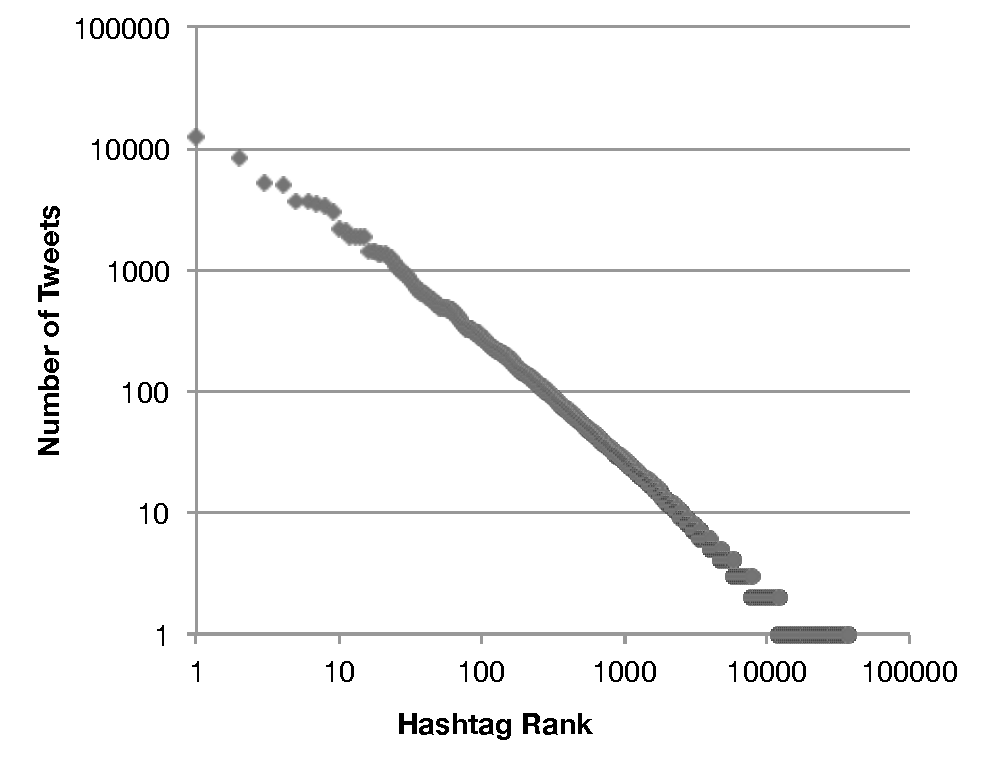
\includegraphics[scale=.5, viewport= 0cm 0cm 16.6cm 12.9cm]{hash-tag-dist.pdf}
\caption{2009 Twitter Hash Tag distribution on a log-log scale.
\label{fig:hash-dist}
}
\end{center}
\end{figure}

The power log scale shows us that there is a large spectrum of subscriber anonymity that can be taken advantage of. Colliding with popular tags gives you plausible deniability as there are relatively few tags dominating the space at a given time, and thus appear as legitimate interests. If there were a more even distribution of tags, then someone observing you following a particular tag would have less incentive to ignore suspicion that your activities might be objectionable to them. \hl{can we get a statistic on what the average number of tags someone follows is?}

\subsection{Collider}

In order to explore the feasibility of steering a particular Plain Tag to collide with an existing Short Tag, we built a collider tool. The tool takes in a Short Tag substring, \textit{T}, a prefix string, \textit{S}, a suffix length, \textit{L}, an alphabet 
\textit{A}. The collider finds the concatenations of \textit{S} and strings of length \textit{L} from \textit{A*} such that the truncated hash of the resultant string matches \textit{T}.

It has two modes of operation. In the default mode, he user specifies some number of tags to return that collide. The collider begins its scan at a random point in the search space and continues scanning until the requested number of tags are found. The second mode scans the entire search space, and therefore returns all matching tags for a given prefix and suffix length.

The search space, then, is of size $|A|^L$. If we wanted to match byte strings, $|A| = 256$, however, we decided to restrict the alphabet to alphanumeric characters due to Twitter's understanding of characters and not bytes, yielding $|A| = 62$. Additionally, the search space can be explored in parallel, giving the Collider executing on a system with \textit{P} processing units, a runtime of $O(\frac{62^L}{P})$.


\begin{figure}
\begin{center}
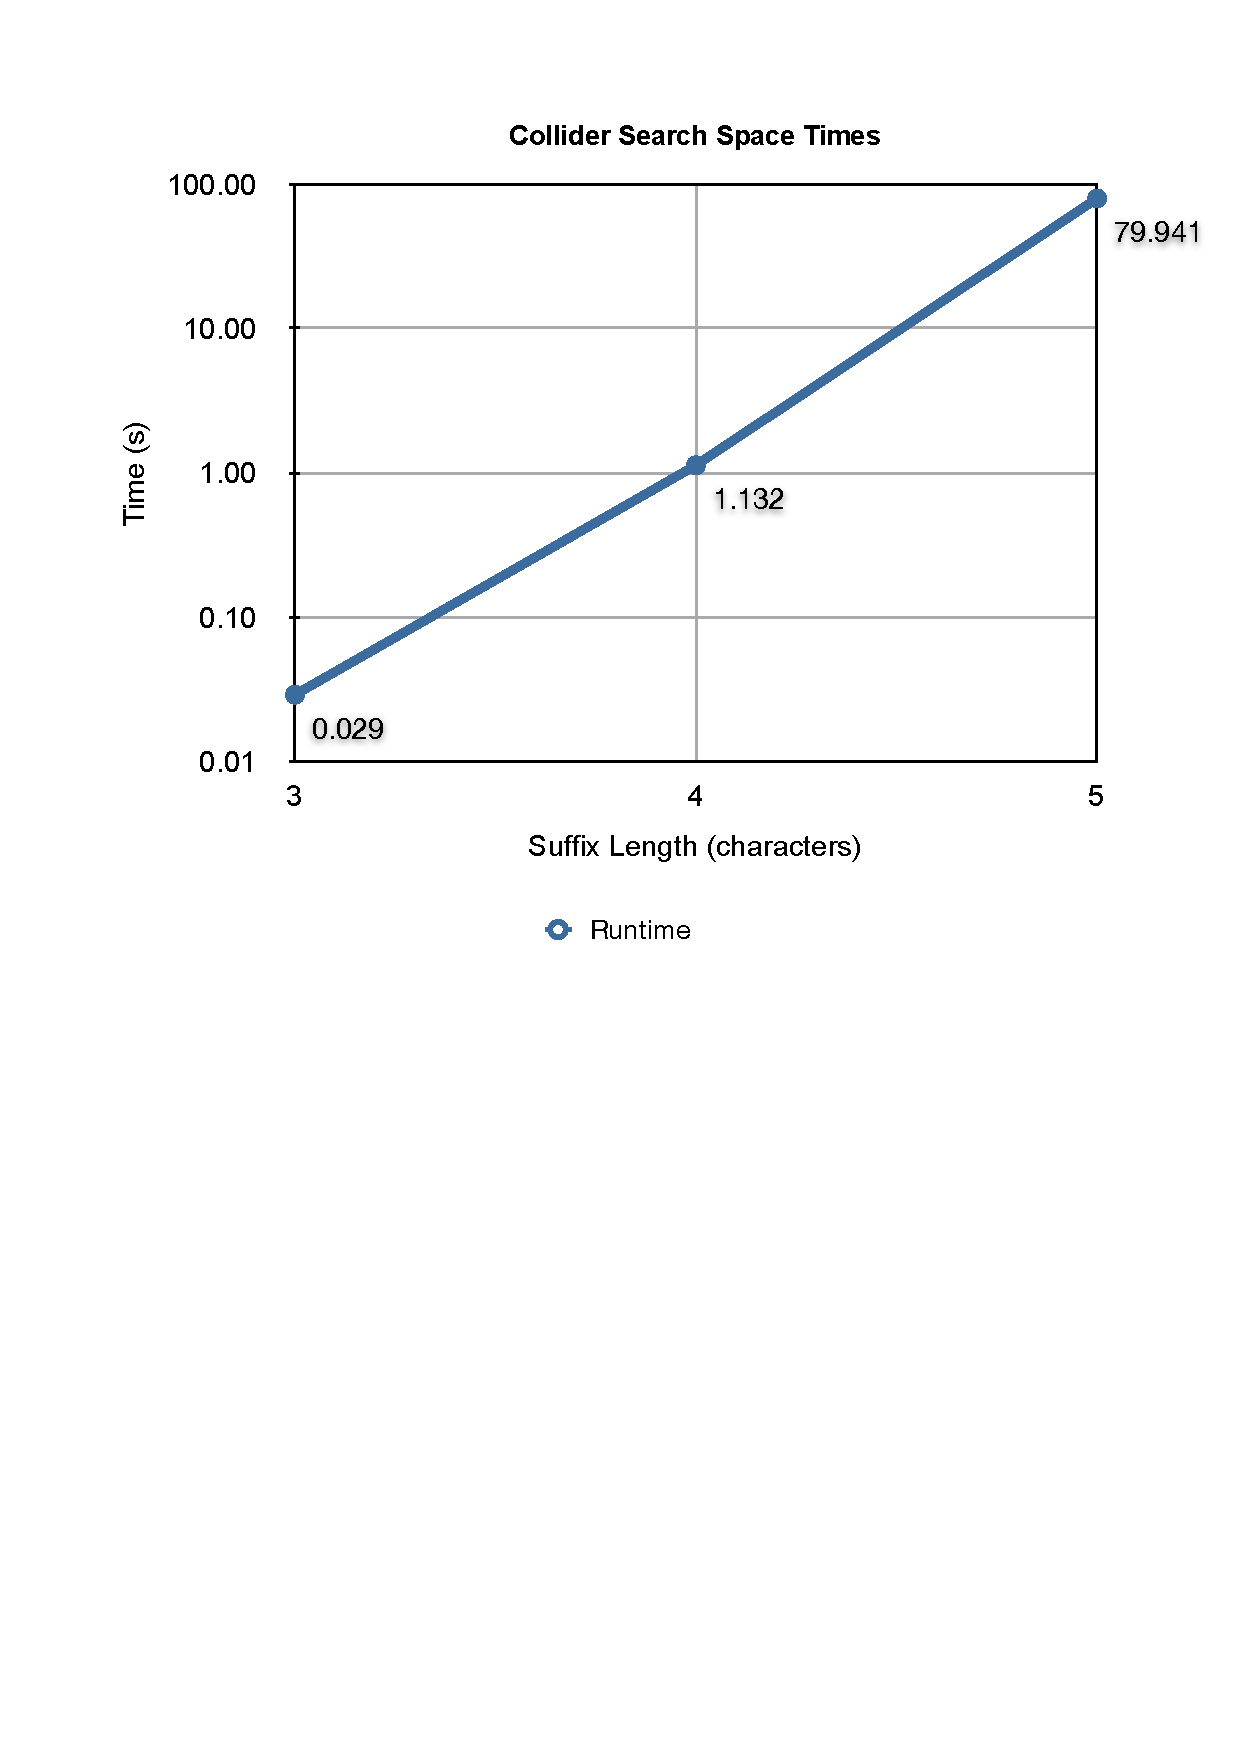
\includegraphics[scale=.5, viewport=0cm 0cm 16.6cm 13.6cm]{collider-times.pdf}
\caption{Runtime for the Collider to search the exploration spaces of sizes $62^3$, $62^4$, $62^5$ on dual quad-core Intel i5 processors.
\label{fig:collider-times}
}
\end{center}
\end{figure}

\begin{figure}
\begin{center}
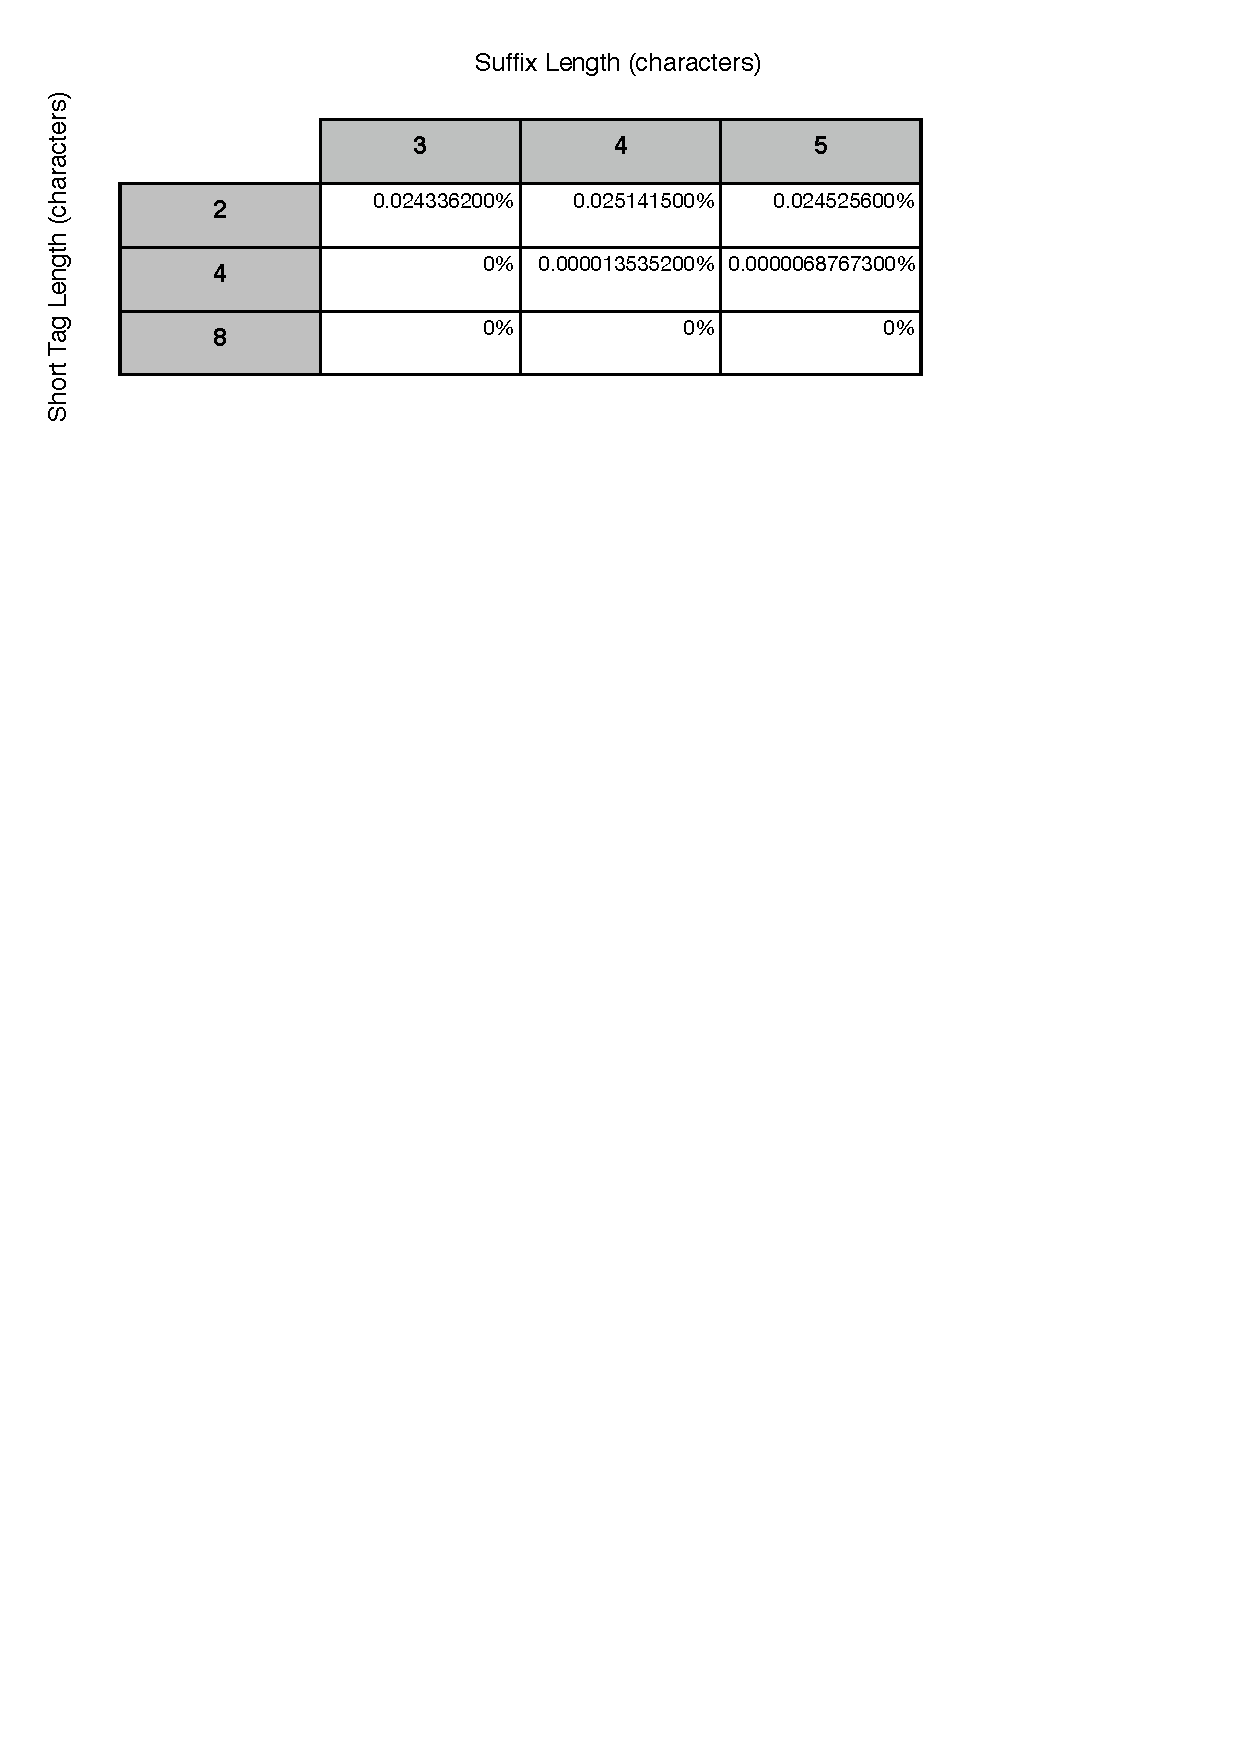
\includegraphics[scale=.5, viewport=0cm 0cm 16.5cm 7.5cm]{collider-hits.pdf}
\caption{Percent of search space that returned hits for an entered Short Tag, with a Prefix of `rice', and given Suffix Length. Length 2 prefix was `Ch', 4 was `Char', and 8 was `CharlieS'.
\label{fig:collider-hits}
}
\end{center}
\end{figure}

As expected, the runtime in Figure \ref{fig:collider-times} scales exponentially with \textit{L}, which in turn it becomes quickly infeasible for a single machine to do an exhaustive search of spaces where the suffix length is greater than 6.

Provided an attacker knows a particular group's prefix and the alphabet out of which they are generating the suffix, the embarrassingly parallel nature lends itself to brute force attacks. If we consider the adversary to be a government for example, it would be fair to assume they have thousands of machines at their disposal for such an attack. It becomes important, then for a user to pick a Plain Tag outside reasonable brute forcing bounds. 

\hl{should the `rememberable' limit discussion go here? or should this paragraph be moved out to discussion?}

Another concern is how easy it is to collide with another tag. From Fig. \ref{fig:collider-hits}, we find that beyond 4 characters, it was impossible to find collisions within easily searchable spaces (suffix sizes < 6). 

The results of these experiments place some limits on what choices a user can make currently regarding anonymity. You can only collide with up to 4 characters in a tag before the search space becomes such that any guarantee of collision is trivially small. Furthermore, $62^6$ is the upper bound on the search space for what a single computer can reasonably calculate a suffix to enable a collision with. Adding one more character to the suffix sends the computation into the span of days on a modern computer at time of writing.

However, we also show that tag collision is possible, there are certainly tunable degrees of anonymity thanks to the apparent power-log distribution of twitter tags already, and finding such a collision is feasibly done on a personal computer. \hl{What more to say here?}

\subsection{Performance}

In this experiment we wanted to see how well the encryption engine performed. In March 2011, Twitter stated that the site receives 140 million tweets per day or 1620 tweets per second on average (http://blog.twitter.com/2011/03/numbers.html). They also said that the maximum tweets per second ever was 6939. These numbers act as rough upper bounds to the number of Hoots per second the system would need to keep up with. In all likelihood, the number of encrypted messages posted would be drastically smaller than regular messages.

The benchmarks in Table \ref{tab:hps} were run on a 1.86GHz Intel Core 2 Duo, 4GB Ram, Macbook Air using Base64 encoding.


\begin{table}
\caption{Average Hoots Per Second for Encryption and Decryption
\label{tab:hps}
}
\begin{center}
    \begin{tabular}{ l  l }
	\hline
	Action & Average Hoots per second \\ \hline
	Encryption & 3614.531 \\
	Decryption & 15587.328 \\ \hline
    \end{tabular}
\end{center}
\end{table}


\hl{computation is negligible. one computer can do it, twittr has more than 1 comp. bandwidth is multiplied by more. more tweets per group. fundamentaly, twitter has to pay this for receiver anonymity. inherent to our scheme. Quantify how much. twitter's bandwitdh bill would go up and they aren't already making money. Cite sandler. people on average send 100 messages and have 100 followers. we dont know how big the groups, we can know how many poeple post, can't know how many listen. After incedient, lots of \#NotAFactualStatement. no idea how many actually listen. Many people could post w/o listening and viceversa. We could treat the numbers as equivelent but that's probbably not a factual statement.Cite: http://www.politico.com/news/stories/0411/53214.html}

Given these numbers, a Twitter server could easily encrypt the entire Twitter feed as the messages were posted. To handle peak usage like the 6939 tweets per second Twitter observed, many optimizations could be made, the simplest being to add a couple computers to help with the load. Our experiment shows that the Hoot protocol does not have significant overhead during encryption or decryption, so it can be adopted with little engineering effort.

It is interesting to note that the decryption rate is important to a client, since a client will be searching tweets trying to identify and decrypt potential Hoots. A client may not trust Twitter to do the decryption since that involves sharing the Plain Tag with Twitter, so a client would decrypt the message on their machine. Almost every client will not have a datacenter of computers for decryption, but our  process can decrypt Hoots almost five times faster than it encrypts them. A client, even with limited computing power, can easily keep up with the Twitter feed.

\hl{Should experiments have a wrap up paragraph?}
\section{Experiments}
\label{sec:experiments}

In this section, we describe the results of our analysis of the \hoot
system with the 2008 Twitter dataset collected by Sandler and
Wallach~\cite{sandler09}. This data contains 10,766,525 tweets with
255,833 hashtag references. Additionally, we show the results of
experiments using our prototype to examine the computational overhead of
implementing \hoot over all Twitter traffic.

\subsection{Cover traffic}
We first show that Twitter groups provide good possibilities for cover
traffic that \hoot can leverage to hide groups seeking plausible
deniability.

In Figure~\ref{fig:hash-dist}, we show the distribution of 
tweet volume for each hashtag in the 2008 dataset, ordered by activity
volume in a log-log scatter plot. The
distribution appears to follow a standard power law distribution, with a
few very active hashtags and many hashtags with few tweets. A large
cluster of hashtags appear only once in our dataset. 

This distribution shows us that there is a large spectrum of subscriber
anonymity set sizes that can be leveraged by \hoot. To get a high
degree of anonymity, a group organizer can choose a plain tag whose short tag
collides with a popular tag (and, thanks to the power-law
distribution, we can be confident there will always be a reasonable
distribution of plain tags, with varying popularity, to choose from).
Among other benefits, a group organizer has the ability to dial in
pretty much any amount of cover traffic for their group.

 % With such a group, the sudden influx of new
% followers will not be as suspicious. Some groups may opt
% for better plausible deniability by selecting a tag that is only
% moderately popular but serves as a believable innocuous interest for
% group members.
%gives
%you plausible deniability as there are relatively few tags dominating
%the space at a given time, and thus appear as legitimate interests. If
%there were a more even distribution of tags, then someone observing you
%following a particular tag would have less incentive to ignore suspicion
%that your activities might be objectionable to them. 

% (dwallach note: plausible deniability is discussed earlier)

\begin{figure*}[t]
\begin{minipage}[b]{0.48\linewidth}
\centering
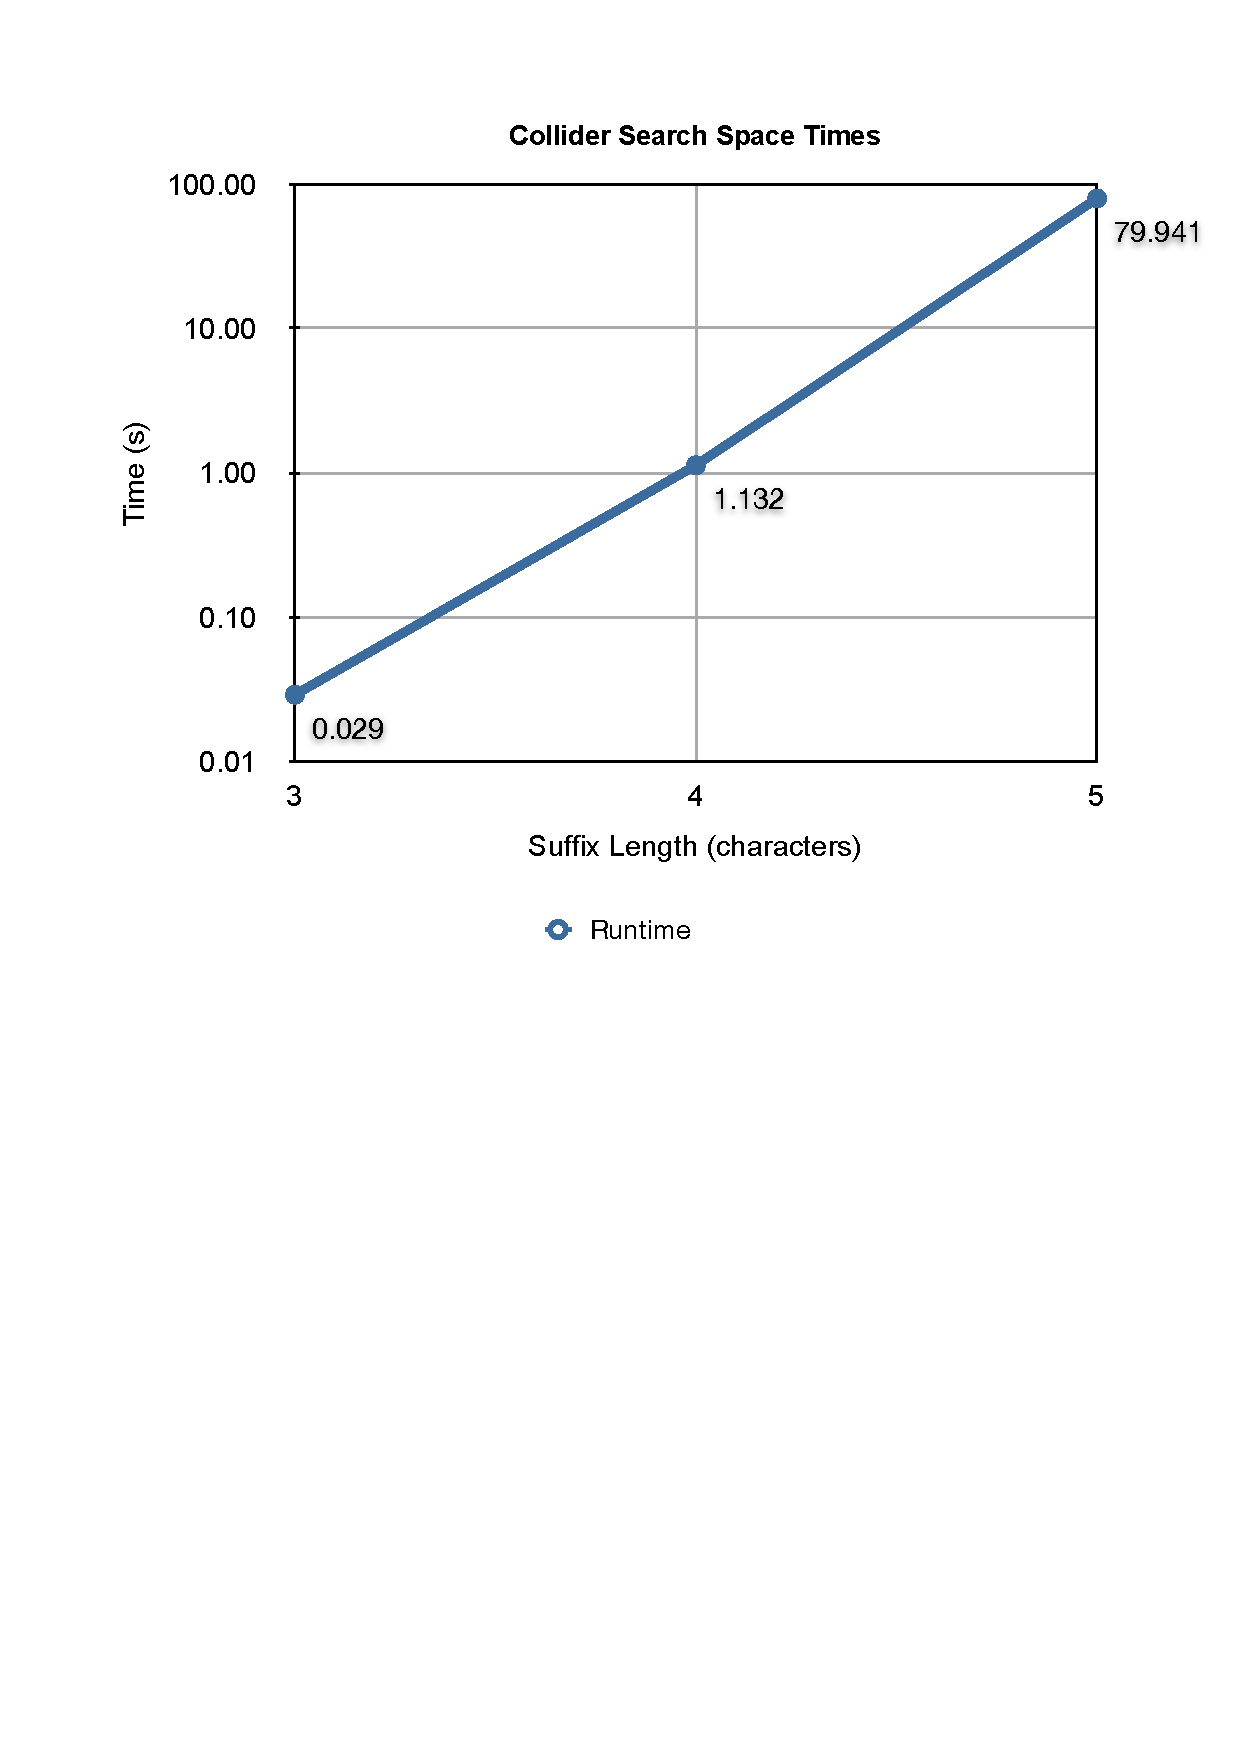
\includegraphics[scale=.5, viewport=0cm 0cm 16.6cm 13.6cm]{collider-times.pdf}
%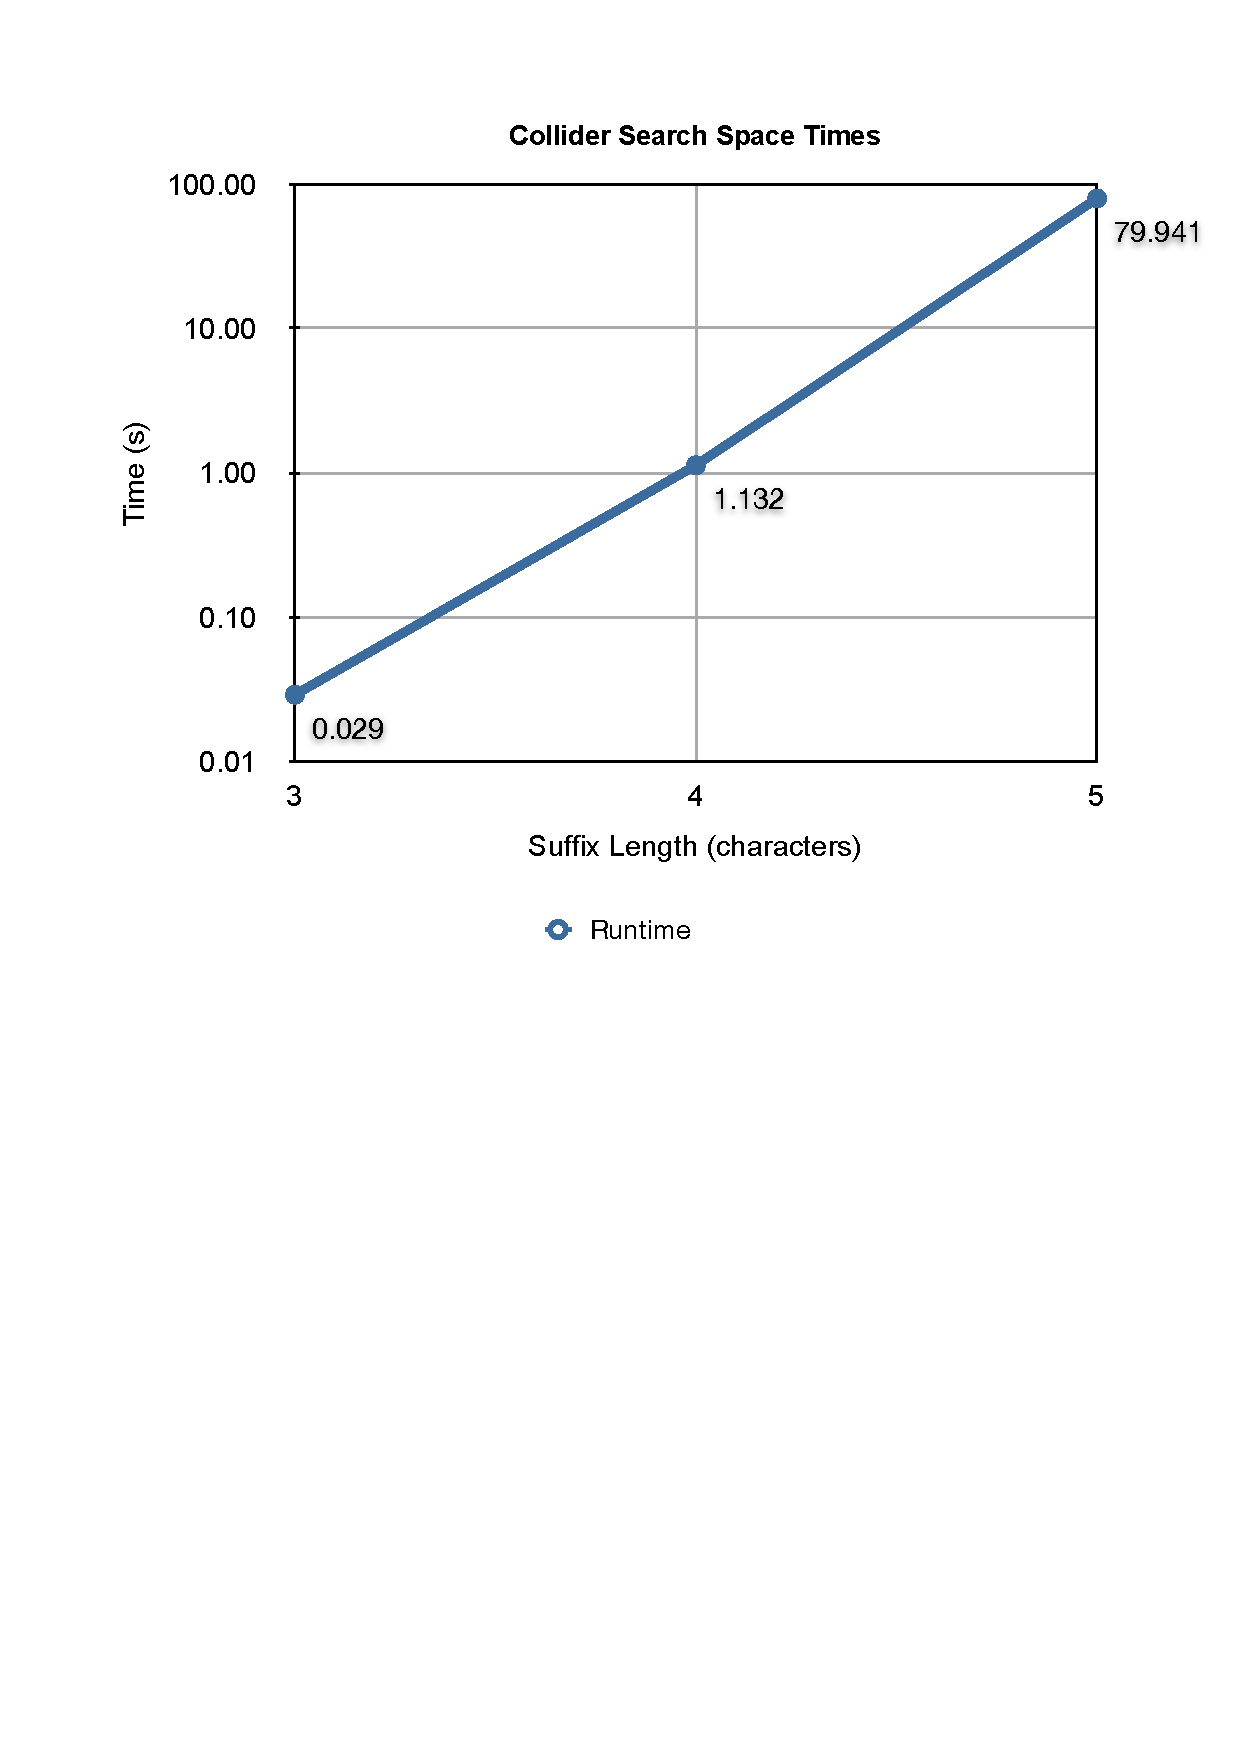
\includegraphics[scale=.5]{collider-times.pdf}
    \caption{Runtime for the collider to search for all matching tags with
  suffixes of length $L=3,4,5$ base-64 digits on a PC with dual quad-core Intel i5
  processors.}\label{fig:collider-times}
\end{minipage}
\hspace{0.5cm}
\begin{minipage}[b]{0.48\linewidth}
\centering
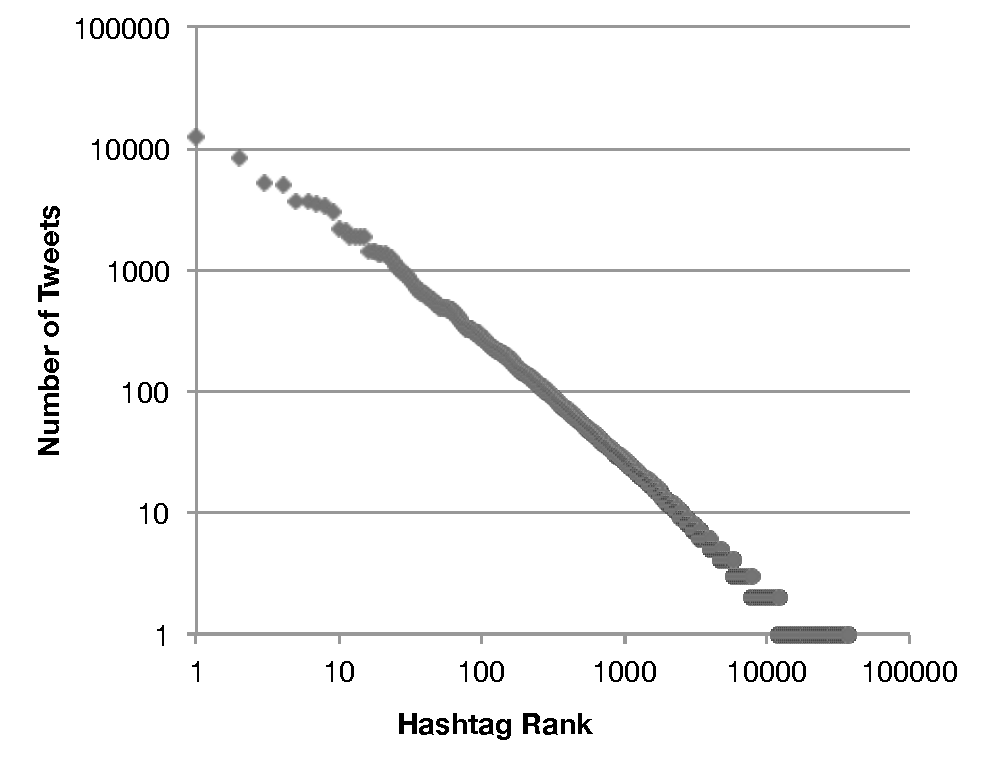
\includegraphics[scale=.5, viewport= 0cm 0cm 16.6cm 12.9cm]{hash-tag-dist.pdf}
%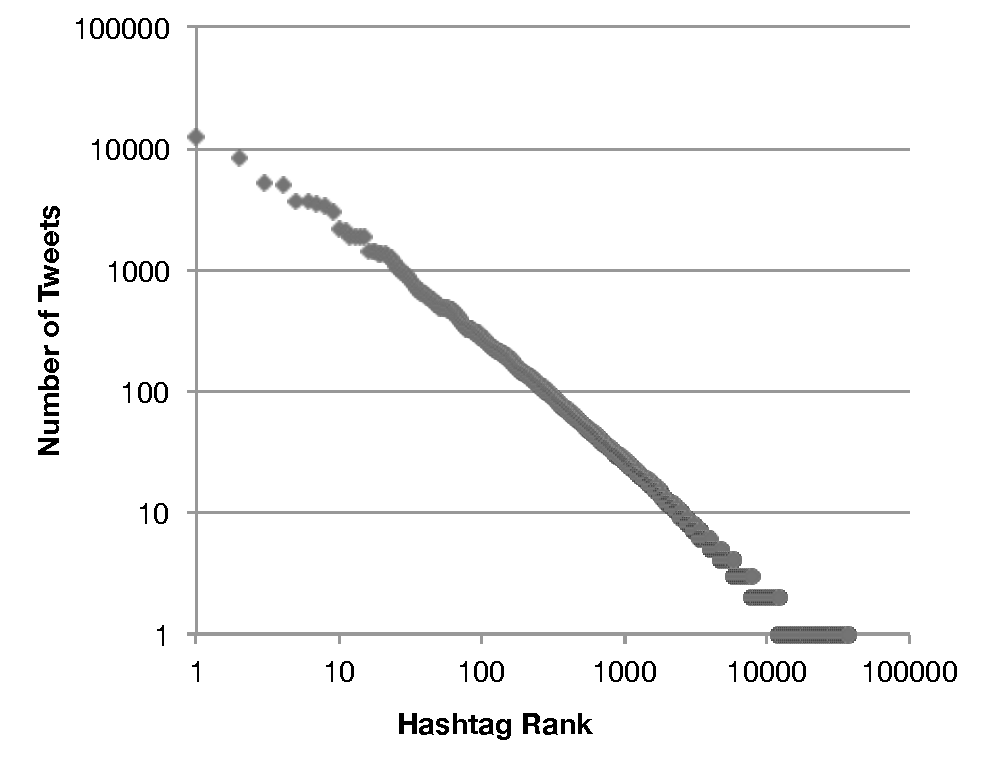
\includegraphics[scale=.5]{hash-tag-dist.pdf}
\caption{2009 Twitter hashtag activity distribution on a log-log
  scale.\vspace{0.4cm}\label{fig:hash-dist}
}
\end{minipage}
\end{figure*}

\subsection{Finding tags}
\label{sec:collider}

To explore the feasibility of finding a plain tag that collides with an
existing short tag, we built a tool called the {\em collider} in C and
OpenMP~3.0, using the open source CommonCrypto\footnote{\url{http://www.opensource.apple.com/source/CommonCrypto/}} library provided
by Apple. The collider implements the \proc{Find-Tag} algorithm
described in Figure~\ref{fig:find-tag} and is trivially parallelizable
by partitioning the search space.

\if 0
The collider takes in a short tag, \textit{T}, a prefix string,
\textit{S}, a suffix length, \textit{L}, an alphabet \textit{A}. It
finds the concatenations of \textit{S} and strings of length \textit{L}
from \textit{A*} such that the truncated hash of the resultant string
matches \textit{T}.

The collider has two modes of operation. In the default mode, the group
organizer specifies the desired number of colliding tags. The collider
begins its scan at a random point in the search space and continues
scanning until the requested number of tags are found. The second mode
scans the entire search space, and returning all matching tags for a
given prefix and suffix length.

The search space is of size $|A|^L$. If we wanted to match byte strings,
$|A| = 256$. However, since Twitter operates on characters and not
bytes, we restrict the alphabet to alphanumeric characters, yielding
$|A| = 62$. We note that the search space can be explored in parallel,
which makes the runtime of the collider executing on a system with
\textit{P} processing units $O(\frac{62^L}{P})$.

% Wow, this really is useless. We need to return the time to find one
% hit. -- dwallach
\begin{figure}
\begin{center}
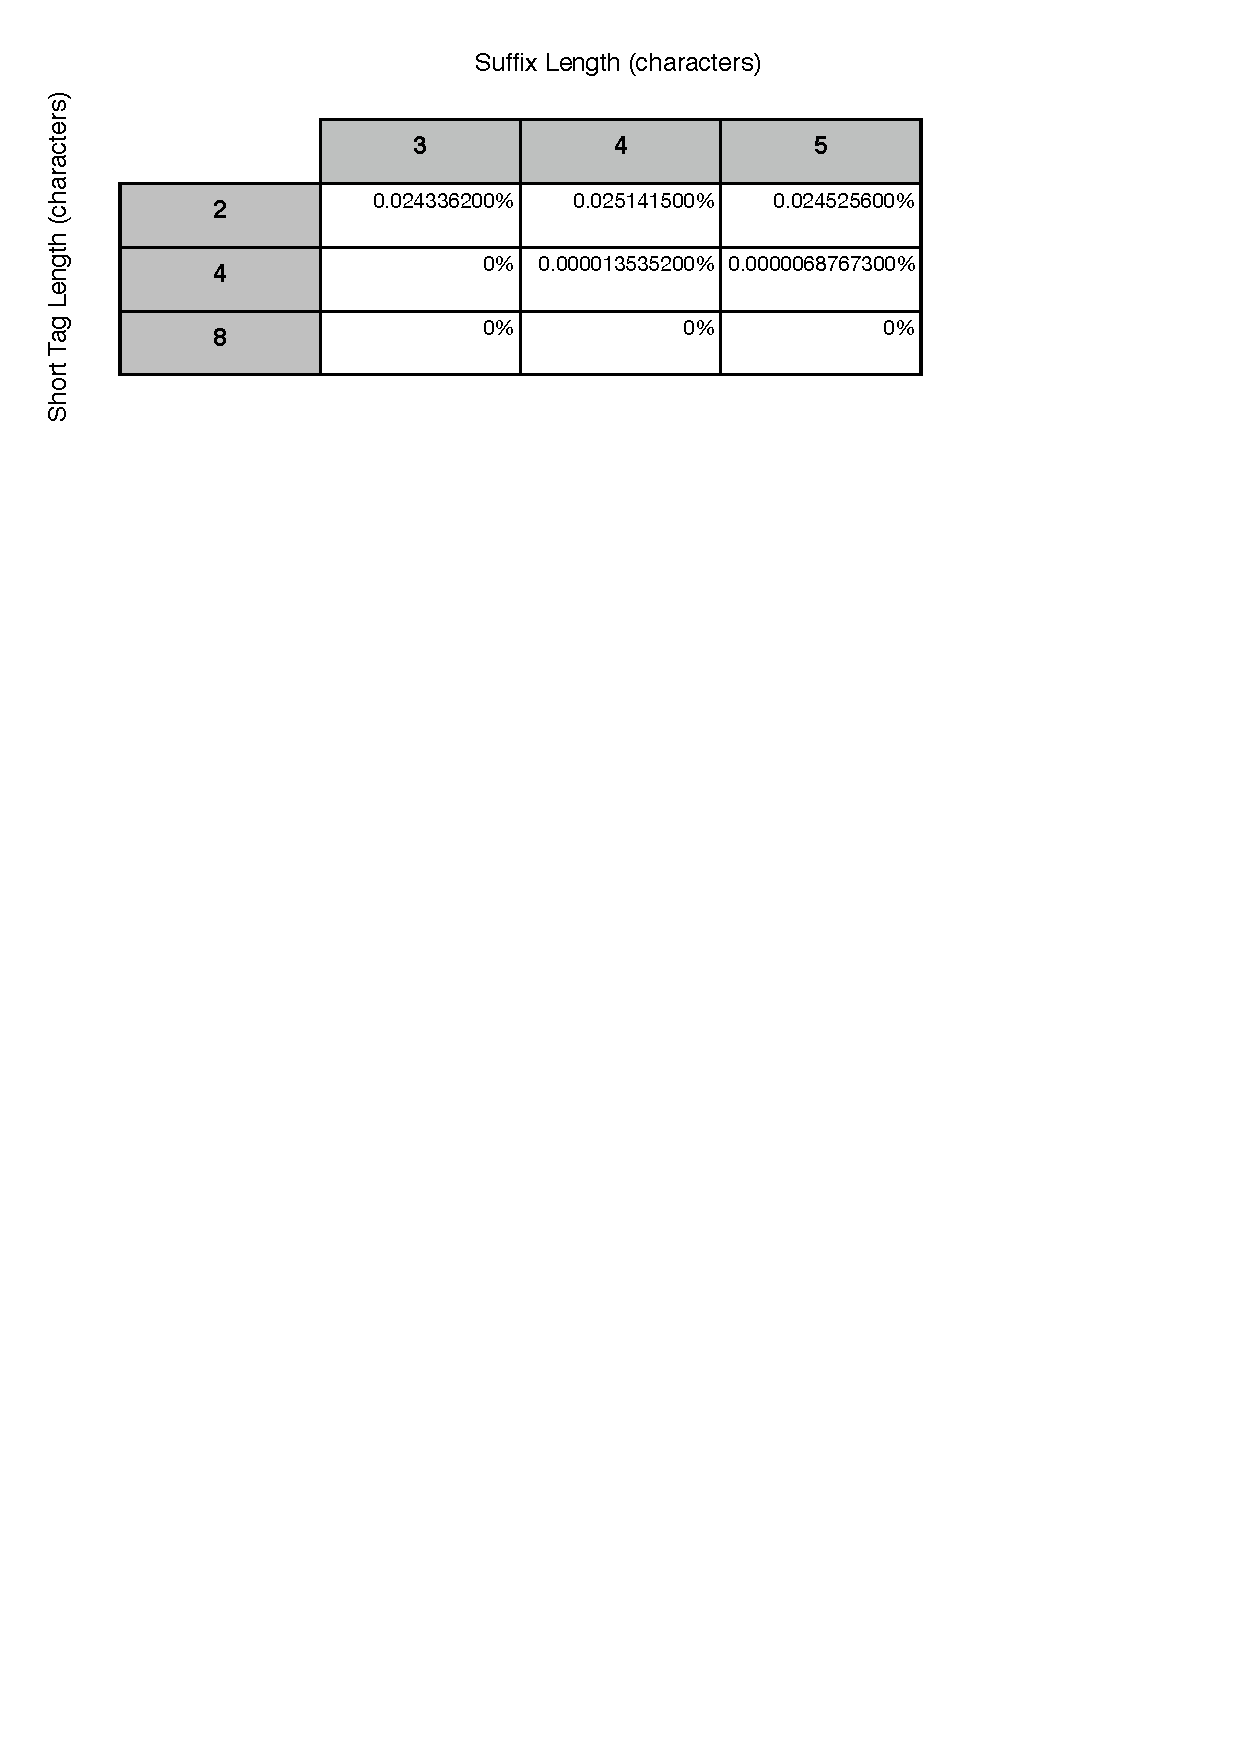
\includegraphics[scale=.5, viewport=0cm 0cm 16.5cm 7.5cm]{collider-hits.pdf}
\caption{Fraction of search space that returned hits for an entered short
  tag, with a fixed prefix and the desired suffix length (in
  Base64). We terminated the computation if no results were found in
  one day of computation.\label{fig:collider-hits}}
\end{center}
\end{figure}
\fi

As expected, the runtime scales exponentially with the length of the
desired collision.  Performance is limited by the performance of SHA-1
of our computer--- roughly 1.9 million ($~2^{21}$) hashes per second per
core.
% dwallach-- measured on my Core 2 Duo iMac -- close enough
% for now.
Consequently, finding a collision in a short tag that's only three
Base64 digits (18 bits) takes a fraction of a second. Finding a
collision in four digits takes only a few seconds. Even with our
parallelized implementation, it is currently infeasible for a single PC
to do an exhaustive search for a suffix greater than six Base64 digits
(36 bits) in less than a day. Note that performance would be slower if
scrypt or any other slow key derivation function was used in place of
SHA-1.

\if 0
%Even if optimizations
%could speed up the calculation, it would likely need to take less than
%an hour to be usable for most groups. On the other hand, finding a
%collision for a short tag is proportional to its size relative to the
%search space.  \hlfixme{FiXme: What about finding one useful suffix?
%  That's the real question...}  \hlfixme{Isn't search time for a single
%  match independent of the search space of the suffix length and
%  dependent on the search space of the short tag length? Or can we not
%  assume even distribution of matching tags? Can I make that argument or
%  am I missing something?}

Another concern is the ability to find colliding tags at all. The
probability $p_{coll}$ of trying $|A|^L$ tags and finding at least one
that has the same short tag as an existing $c$-character tag is given
by:
%
\[p_{coll} = 1-\left(1-\frac{1}{|A|^c}\right)^{|A|^L}.\]
%
For an alphabet of $|A|=62$ glyphs and a short tag length of $c=2$, a
suffix of $L=3$ characters is enough to nearly guarantee at least one
collision. For a short tag length of $c=4$, a suffix of $L=5$ is
required. 
% mkw -- I can't figure out the general formula.
% The 
% \hlfixme{Numerically, on my calculator, I notice that for
%  A=62, L=c will give you prob. 0.643, and L=c+1 gives you very
%  tiny. That's not a coincidence -- find the correspondence.}

To validate this analysis with real tags, we studied the number of
collisions we could find for various values of $c$ and $L$ for a
specific prefix (``rice'') and fixed short tag values. The results,
shown in Figure~\ref{fig:collider-hits}, confirm that short tags of
length four require a suffix of length four or more to find a collision.

Thus recipient anonymity is attainable for short tags of length four or
less, and tied to this is recipient deniability. The more innocuous
traffic that is pulled, the more it seems as if you are truly following
some hot topic, rather than a more clandestine group. An observer
monitoring the tweets you download will be unable to differentiate
someone following a secret group and someone following a popular topic
because members of both groups will pulling all \msgs from each other's
groups.
\fi

%how easy it is to collide with another tag. From
%Fig. \ref{fig:collider-hits}, we find that beyond 4 characters, it was
%impossible to find collisions within easily searchable spaces (suffix
%sizes < 6).

%You can only collide with up to 4
%characters in a tag before the search space becomes such that any
%guarantee of collision is trivially small. 
%Furthermore, $62^6$ is the upper bound on the search space for what a
%single computer can reasonably calculate as a suffix to enable a
%collision. Adding one more character to the suffix sends the computation
%into the span of days on a modern computer at time of writing.
%
%However, we also show that tag collision is possible, there are certainly tunab%le degrees of anonymity thanks to the apparent power-log distribution of twitte%r tags already, and finding such a collision is feasibly done on a personal com%puter. \hl{What more to say here?}

\subsection{Overall \hoot performance}

Adoption of \hoot requires that the overhead for encryption and
decryption be minimal. For example, one path to adoption would have
Twitter or another microblogging service offer \hoot semantics over
their entire existing service. We thus consider computation overhead in
the context of encrypting {\em all} Twitter traffic as a worst case. In
March 2011, Twitter stated that the site receives 140 million tweets per
day or 1620 tweets per second on
average\footnote{\url{http://blog.twitter.com/2011/03/numbers.html}}. Twitter
also stated that the maximum number tweets per second ever was
6939. These numbers act as rough upper bounds to the number of hoots per
second the system would need to keep up with.
% In all likelihood, the number of encrypted
% messages posted would be drastically smaller than regular messages, at
% least in the early deployment of \hoot.

\begin{table}
\caption{\hoot computation rate for encryption and
  decryption.\label{tab:hps}}
\begin{center}
    \begin{tabular}{ l  r }
	Action & Average hoots per second \\ \hline
	Encryption & 3610 \\
	Decryption & 15590 
%	Encryption & 3614.531 \\
%	Decryption & 15587.328 \\ \hline
    \end{tabular}
\end{center}
\end{table}

To study the amount of computation required to support \hoot over
Twitter, we modified our Python script to perform the encryption process
500,000 times running on a MacBook Air with a 1.86~GHz Intel Core~2 Duo
using Base64 encoding to demonstrate how the performance would be on a
typical end user's laptop. This also gives us a lower bound for
performance on modern hardware. We also independently performed the
decryption process 500,000 times.  Table~\ref{tab:hps} demonstrates that
the computational overhead for \hoot cryptography is negligible for
Twitter; the average computational load can be handled by a single
computer and the peak load might require only two computers. Clearly,
the issue for Twitter or a comparable service wouldn't be cryptographic
costs, it would be bandwidth. That overhead would be entirely dependent
on the selection of the short tag on the part of the various \hoot
organizers.

On the client side, our experiments show that a modern computer can
decrypt \msgs significantly faster than Twitter's peak message rate for
the entirety of its traffic. (Even better, the MAC can be validated
before the message ciphertext needs to be decrypted, providing a
shortcut to skip undesired cover traffic.)  Again, computational
overhead isn't going to be the limiting factor.  Instead, the only issue
will be bandwidth.

Group organizers must then take client bandwidth into account when
selecting collisions. An international pop music star might make for an
excellent cover story, but he might simply be too popular for clients,
particularly if the they are using cellular phone networks that haven't
been brought up to the latest multi-megabit speeds.  This is the one
place where the short size of Twitter messages actually works in our
favor. A modest data pipe of 128 kbits/sec can transmit roughly 114
tweets per second. This is well within the regular bounds of most any
short tag selected by the group organizers.

Assuming the entire peak load 7000-or-so tweets per second ends up split
uniformly across short tags with three base-64 digits (i.e., 18 bit
short tags), the average number of tweets per second per short tag is
only 0.02 (i.e., only 1.6 \msgs per minute). That's well within any
realistic bandwidth constraint.


\if 0


The decryption rate is important to clients, since clients will need to
search through hoots with colliding hashtags and decrypt the session
keys for each one to see if it decrypts correctly. Note that, with a
simple fixed constant string prepended to the keys, the client can
quickly verify whether the message was encrypted using $k_{tag}$ or if
another group's key was used. Since our process can decrypt Hoots almost
five times faster than it encrypts them, even clients with limited
computing power can keep up with the entire Twitter feed. In practice,
clients would only need to decrypt hoots that share the same short tag,
which should be a small fraction of this cost even for very active
groups.

%A client may not trust Twitter to do the decryption since that involves
%sharing the plain tag with Twitter, so a client would decrypt the
%message on their machine. Almost every client will not have a datacenter
%of computers for decryption, but 
%adopted with little engineering effort.

%\hl{Should experiments have a wrap up paragraph?}

%\hlfxnote{mkw -- I don't think so. We'll cover more ground in the discussion.}

\fi

%\section{Discussion}

In this section, we discuss a variety of issues and future extensions of the Hoot design.

\subsection{Incremental Rollout}

\hl{
1. Can you incrementally roll it out
	- Service provided by twitter or yourself
2. 140 character limit
	- Twitter doesn't have to go too far to have all the metadata for encryption
	
	- How hard is it for twitter to do this. 
	- Reference message fitting into 140 char using unicode
	- Reference peak hps, and how our system holds up
}
\subsection{Adoption}	

The next question to ask after we have shown that rolling out the Hoot service is feasible would be whether Twitter would actually implement such a feature. Based on the nature of Twitter, we believe that Twitter would not add a secure messaging framework like Hoot. Twitter as a company needs to know what people are talking about, so it can provide relevant advertisement. Adding the Hoot infrastructure to Twitter would prevent Twitter from knowing the content of the messages, and so we believe the Hoot service will never be adopted. However, this need not prevent individuals from using the Hoot protocol over Twitter. As long as Twitter faithfully delivers tweets, users are free to run the Hoot encryption on their own machines over their messages and then post the output to Twitter. In fact, this method is more secure in that a user only has to trust their machine. If Twitter is responsible for encrypting a message, nothing is stopping them from keeping a copy of the plain text message. Paranoid users will always want to encrypt messages themselves, so Twitter adopting the Hoot protocol is unnecessary.
		
\subsection{Usability}

As described in the Cover Traffic section, a group can deliberately collide with a popular tag by concatenating an easily rememberable string of text with random letters or numbers. As Miller\cite{miller56} noted, people can remember  
7 +/- 2 unique packets of data, so as long as these collisions can be generated with a suffix in that range a user is likely to be able to remember it. We could further improve rememberability by restricting suffix values to only digits, and then generate a suffix of 7 or 10 digits, emulating a phone number. The main requirement is that a group should be able to have a unique shared secret that can deliberately collide with other tags while still being easy to remember and more importantly easy to transfer. Since our proposal does not deal with key transfer, we assume our key communication is done through whisper channels and thus must be short and memorizable for simple transfer. We have found that a collision can be found with only appending 3-6 characters to a prefix, so deliberate collisions can both be found and transferred without much effort.

\hl{
-- Entropy 7+-2
-- Deliberate posting crap (to hide your stuff).
-- Increases work factor (signal to noise)
-- Fairly strong attacker, but user who don't have ability for a lot of entropy
-- 70 bits is enough compared to the weakness of everything else
}
\subsection{Alternate Backends}

Even though our protocol was designed with Twitter in mind, it is extensible to other systems and platforms. The Hoot protocol describes a secure way to transfer short messages (with short encryption overhead) across a publicly available network completely openly. Twitter is a great example of this environment but not the only one. Hoot could interact, for example, with a Distributed Hash Table system (DHT) like CHORD or Pastry. Importantly, Hoot can interface with both centralized systems like Twitter or Buzz or decentralized systems. As long as the platform's content is publicly searchable, the Hoot protocol allows secure transmission to anonymous group followers.

\hl{Discuss how we can make it harder for an attacker. Maybe hashing 1000 times...}
\section{Discussion} \label{sec:discuss}

In this section, we discuss a variety of issues and future extensions of the \hoot design.

\subsection{Deployment}

There are two different paths through which \hoot could be deployed. First, it would be straightforward to implement a proxy service, whether operated by Twitter or by an independent third party, that reads every tweet, encrypts it, and provides a Twitter-like interface to the stream of \msgs. This would incur non-trivial monetary costs for the bandwidth and computation resources, but it is still well within the means of many organizations. A deeper concern is that any country could simply block traffic to or from the \hoot proxy server.

Alternately, the proxy server could read every normal tweet, encrypt it, and post it back to Twitter. This, naturally, would double the number of tweets, which makes it something that Twitter would probably insist on doing themselves rather than accepting from a third-party service. A Twitter-internal implementation might instead, for example, precompute the short tags for every tweet but regenerate \msgs on the fly rather than storing two copies.

Any strategy in which \msgs are injected by a proxy has the property that the \msg need not necessarily specify the original sender's Twitter username.  Breaking the binding between the sender and the public \hoot message would greatly improve sender anonymity, but it would also allow any user who knows the relevant plain tag to impersonate any other member. We could imagine a variety of ways to add some sort of digital signature or hash-chaining layer into the \msg format to differentiate users with ``read-only'' versus ``posting'' privileges. We leave this for future work.

Regardless, a critical question is whether the plain tag for a \msg should ever be sent to Twitter. For users with dedicated clients, the users' plain tags could be stored locally, avoiding any issue where a compromise of Twitter's server becomes a single point of failure for \hoot's confidentiality and integrity. This would clearly be the preferred modality for \hoot usage, but that may not be feasible for a large number of potential \hoot users.

It's important to note that Twitter's web interface offers full SSL encryption. Twitter's dedicated smartphone clients currently use OAuth signatures, protecting message integrity but not privacy. Full encryption would be desirable for smartphone clients to defeat active adversaries who might use deep packet inspection to detect \hoot messages in transit and close the connection.

A few other considerations are worth noting:
\begin{itemize}
\item If Twitter could be convinced to directly support \hoot, then they could certainly stretch the 140-character limit to allow \hoot plaintext messages to be as long as regular Twitter messages.

\item If \hoot users were connected to Twitter's web interface, then it would be essential for \msgs to be decrypted in the browser, via client-side JavaScript, rather than on the server. We want every \msg matching a short tag query to be transmitted over the network to ensure that passive network eavesdroppers, will only see traffic patterns corresponding to those short tags. Sending just the \msgs matching a particular plain tag could leak the group's traffic pattern, even over an SSL-encrypted connection~\cite{liberatore06}.

%, thereby leaking .
%, which leaks nothing useful, versus particular plain tags, which would elimina%te any cover traffic and thus leak valuable information to the adversary.

\item Regardless, an adversary conducting traffic analysis might be able to distinguish a subscription to a \hoot short tag from a subscription to something else, solely based on \msgs' timing and size. This could be addressed by having {\em all} Twitter users receive \hoot cover traffic for a randomly selected \hoot short tag, which their clients would then ignore. It could also be addressed by hacking normal Twitter clients from unsuspecting users to treat any request to follow a hashtag by having them follow the corresponding \hoot short tag, instead.

\item At some point, Twitter may deploy content-aware advertising on its services. Advertising should never be allowed to operate based on a decrypted \hoot, as the advertiser could well be the adversary, and could possibly use analysis of advertisement metrics to violate \hoot users' privacy.

\item Twitter may not have any interest in \hoot or anything like it. See Section~\ref{sec:dht} for a discussion of alternative backend designs.

\end{itemize}



\if 0
Twitter would not need to go far to have all the metadata necessary to encrypt and decrypt for their users. They would need an interface to allow users to mark a tweet as encrypted, and everything in the tweet would bee encrypted using the hashtag in the message as the plain tag. As we showed previously, fitting into the 140 character limit is possible with Unicode encryption, but Twitter could easily make an internal exception for \hoot. We also showed that computation for encryption and decryption is negligible. One computer can do it, and Twitter has entire racks of computers. The real issue is how the \hoot system would affect bandwidth for Twitter. The bandwidth would increase based on the group collisions and the number of Hoots to a group. Users no longer follow a single tag and read everything. They subscribe to a Short Tag, which collides with many other groups, and therefore they must see all the noise of the other groups on their Short Tag. Fundamentally, Twitter has to pay for the receiver anonymity inherent in the \hoot protocol. 
% mkw -- looks okay. 
%\hlfixme{Someone double check this reasoning:} 
For $N$ groups who collide onto $S$ Short Tags with each group posting $M$ messages, the added bandwidth would be $M\frac{N}{S}$ as opposed to the original bandwidth of $M$. This accounts only for group messages, when in reality there are many more tweets that do not have hashtags. The bandwidth additions for \hoot might be very small compared to the bandwidth used to send ordinary non-group messages.

According to Sandler and Wallach~\cite{sandler09}, Twitter users, on average, send 100 messages and have 100 followers. It is difficult to know how many groups (hashtags) users post to, but it is even more difficult to know how many users listen to a particular group. After Sen. Jon Kyl made an inaccurate statement, his spokesperson cleared it up by saying it was ``not intended to be a factual statement''~\cite{politico11}. Stephen Colbert then encouraged his followers to tweet using the hashtag \#NotIntendedToBeAFactualStatement. This quickly became a popular Twitter group, but it is impossible to know how many people were actually listening to the group but not posting. Even those posting to the group might not be listening to all the other tweets to the group. We could treat the number of posters and the number of listeners as equivalent, but that is not intended to be a factual statement.

Regardless of the number of groups or Short Tags, Twitter's bandwidth bill would certainly go up, and since their finances are already dubious, implementing \hoot may be a concern.

\subsection{Adoption}	

The next question to ask after we have shown that rolling out the Hoot service is feasible would be whether Twitter would actually implement such a feature. Based on the nature of Twitter, we believe that Twitter would not add a secure messaging framework like Hoot. Twitter as a company needs to know what people are talking about, so it can provide relevant advertisement. Adding the Hoot infrastructure to Twitter would prevent Twitter from knowing the content of the messages, and so we believe the Hoot service will never be adopted. However, this need not prevent individuals from using the Hoot protocol over Twitter. As long as Twitter faithfully delivers tweets, users are free to run the Hoot encryption on their own machines over their messages and then post the output to Twitter. In fact, this method is more secure in that a user only has to trust their machine. If Twitter is responsible for encrypting a message, nothing is stopping them from keeping a copy of the plain text message. Paranoid users will always want to encrypt messages themselves, so Twitter adopting the Hoot protocol is unnecessary.
\fi
		
\subsection{Usability}

In essence, \hoot requires its users to manually negotiate a group cryptographic key management system. Even though the use case for \hoot looks and feels much like ``normal'' Twitter hashtags, we are still putting a non-trivial amount of trust into a protocol that requires users to use literal gossip to spread key material. Even highly motivated users could well make mistakes, and any small error would result in the inability to decrypt the desired \msgs. In particular, a significant amount of entropy is required for adequate security, causing \hoot plain tags to push the boundaries on human memorability. In effect, a good \hoot plain tag is comparable to a strong account password. \hoot's use of machine-generated plain tags would have comparable issues with organizations that require users to have strong passwords that are never written down and frequently changed.  And, unlike such organizations which can adopt a variety of ``two factor'' authentication technologies to reduce their reliance on passwords, \hoot fundamentally needs plain tags as strong as strong user passwords.

About the only good news in this process is the growing ubiquity of smartphones, typically having a variety of methods to communicate with other phones nearby. This would allow a set of plain tags to be quickly and painlessly shared via means including two-dimensional barcodes (displayed on one phone's screen, read with another phone's camera), a variety of close-range networking technologies (near-field communication, Bluetooth, ad-hoc WiFi, or infrared file transfer), or even acoustic transfer from one phone's speaker to another phone's microphone. If, in fact, the predominant modality for \hoot plain tag sharing is one of these mechanisms, then plaintag memorizability becomes a non-issue. Plain tags can then be implemented with general-purpose securely-chosen random numbers.

A related usability question is the process for selecting the desired
external hash tag with which to collide a \hoot plain tag. Earlier in
this paper, we cavalierly suggested that famous pop singers helpfully
provide all the cover traffic we might ever want. However, this process
ultimately needs to be handled with care, since recipient deniability
requires the human recipient to have a convincing story under coercive
pressure, and many people may not be able to convincingly demonstrate
their admiration for an overseas pop sensation. A \hoot proxy or other
site could facilitate this by providing information about the popularity
of different short tags, including which ones are trending well in a
given country or region.
%The selection of a
%suitable Twitter hashtag for \hoot collisions would benefit from a
%dedicated web site, engineered for this specific purpose. 
%Naturally, a censorship-happy country will do its best to block access
%to such a web site, requiring group organizers to leverage Tor or
%otherwise be resourceful enough to connect to the outside world.

\if 0

As we described in the Cover Traffic section, a group can deliberately collide with a popular tag by concatenating an easily rememberable string of text with random letters or numbers. As Miller~\cite{miller56} noted, people can remember  
7 +/- 2 unique packets of data, so as long as these collisions can be generated with a suffix in that range a user is likely to be able to remember it. We could further improve rememberability by restricting suffix values to only digits, and then generate a suffix of 7 or 10 digits, emulating a phone number. The main requirement is that a group should be able to have a unique shared secret that can deliberately collide with other tags while still being easy to remember and more importantly easy to transfer. Since our proposal does not deal with key transfer, we assume our key communication is done through whisper channels and thus must be short and memorizable for simple transfer. We have found that a collision can be found with only appending 3-6 characters to a prefix, so deliberate collisions can both be found and transferred without much effort. By brute-forcing to find a collision, the string of characters after the prefix  can be considered "random." Yan et. al~\cite{yan00} discussed random and mnemonic passwords. Our string of characters will rarely be mnemonic, so it suffers from the issues they mentioned like users forgetting the password, but on the other hand random passwords are stronger than mnemonics as shown by Kuo et. al.~\cite{passwords06}.

To make the system even more usable, the client or Twitter should automatically find groups for the user to collide with rather than the user finding it by hand. This system could even allow the user to tweak a parameter for how active a group to collide with.
\fi


%For some users, it may be appropriate for the client to search twitter
%characteristics of the groups with which the user wants the collision,
%e.g. the activity level of the groups and

\subsection{Adaptability and scalability}

Since \hoot benefits from and encourages collisions in the short tag
space, there will come a point when there are simply too many
collisions, i.e., the ratio of desired messages to cover traffic will
eventually become too small to be practical for the proxy or client
software to decrypt and filter through. The seemingly obvious solution
is to adjust the length of short tags. Adding one character to the tag
length would greatly decrease the chance of random collisions (by
$\frac{1}{|A|}$ for alphabet $A$). However, modifying the tag length
while the system is in use would not be straightforward for
groups. Groups could rely on group leaders to facilitate the process,
e.g. by announcing a new tag to use or giving out multiple plain tags in
advance. Alternatively, the system operators could initially set tags to
be long enough to prevent most random collisions and have groups
emphasize chosen collisions in their plain tag generation.

%Doubling the number of possible short tags reduces the number of
%collisions in half it would anyway, since the , or at least it would if
%there were a uniform distribution of raw traffic across the space of
%short tags.
%Given how a small number of hashtags can become hot, trending topics,
%it's far from obvious how changing the standard short tag length would
%impact the distribution of message, nevermind the pragmatic concerns
%with keeping every user on the same page when the short tag length is
%supposed to change.
%
%This process would benefit from the active engagement of group organizers. Cons%ider the case where a low-volume group organizers selects a low-volume plain ta%g with which to collide. Everything works great until some heretofore unseen ha%shtag suddenly rockets to the top of Twitter's trending discussions and just ha%ppens to collide with the very same plain tag. Our group organizers would need %to stay on top of these issues, with a migration strategy ready to go. Option \%#1: implement a command to migrate to a new plain tag which could be broadcast %in the message body of a \hoot; this would, of course, require some way of auth%enticating the command. Option \#2: group organizers would give out multiple pl%ain tags, far in advance, allowing them to issue a suggestion that the group is% moving from plain tag \#1 to plain tag \#2.

\if 0
messages  there will be too much noise to signal for a specific group when following an identifier that collides with many groups. At some point, the entire Hoot universe will want to decrease the amount of collisions. The simple solution is to increase the Short Tag length. Whenever there is too many collisions, the Short Tag length will be increased by one, which will result in far less collisions until the communication increases and eventually the cycle continues. 

The nature of Hoot makes it convenient for this Short Tag length tuning to be done at the system level or at the group level. For instance, a group that is overrun with collisions with popular group could simply increase their Short Tag length internally. All Hoots would include the extra character in the Short Tag, and all subscribes would search for the longer Short Tag. It is also as simple for the entire system to switch to a longer identifier by having an ``oracle'' broadcast to everyone that the system Short Tag length has increased.

Even in a distributed system where some users may not receive the oracle's broadcast, the system still functions. For example, assume user $A$ is following a group who's Long Tag begins ``A5trxq...'', and in $A$'s view, Short Tags should be 2 characters. For user $B$, who posts messages to the group, the Short Tag length should be 3. $B$'s Hoot would then look like ``\#A5t'', but $A$ would be searching for ``\#A5". Twitter's search functionality will still return $B$'s messages for $A$'s search. Although $A$ will be getting much more noise than signal when they search at the shorter length, they will not miss any Hoots.

Previously, we stated that a Short Tag is the first K bytes of the Long Tag, so we explicitly put a limit onto how long a Short Tag can be. Does this prevent us from adapting to an ever growing Hoot ecosystem? In our implementation, we use the first 16 bytes of the Long Tag for identification. Therefore using Base64 encoding, we get $62^{16}$ or $4\times10^{28}$ unique identifiers. In a system with 16 byte Short Tags, there would rarely if ever be collisions, much less too many collisions to increase the length.

Finally, as a result of the encoding systems, the size of the Short Tag space increases by a large factor for each character added. This takes a space that is highly populated to a space that is very sparse, so it is very possible that by adding one character to tag identifiers that groups would be uniquely identified. Groups that also deliberately collided with another group would often not collide at a longer Short Tag length. It would be convenient to instead grow the space by single bits at a time, so as to double the space, a much smaller factor. Unfortunately, Twitter is a character driven environment rather than bit driven, so this is difficult to address. It also does not deal with deliberate collisions. All deliberate collisions will need to be regenerated after a Short Tag length increase.
\fi


% \hl{
% chris 
% - need a citation for core growth so we can make argument about whether searching will keep being feasible
% - twitter vs moore
% - need a citation, or argument, for how fast we expect twitter to grow in the future, can we turn the nob slow enough to keep in pace with processing power, and still be usable? 
% }

\subsection{Alternate backends}
\label{sec:dht}

Even though our protocol was designed with Twitter in mind, it is extensible to other systems and platforms. The \hoot protocol describes a secure way to transfer short messages (with low encryption overhead) across virtually any publicly available content distribution network. All that \hoot requires is efficient search primitives for each message's short tag or tags. Everything else is handled by client-side software.

Consequently, if Twitter had no interest in \hoot or concluded that it would not be supportable, then \hoot could just as easily work with a variety of centralized or distributed network services. To pick one possibility, \hoot could use the BitTorrent ``distributed tracker'', or any other large and public distributed hash table (DHT) service, to store messages with the short tags used to name the DHT nodes responsible for their storage. FeedTree~\cite{sandler05feedtree} is one of many systems that have attempted to support micropublishing on a DHT. (Other DHT-based ideas are discussed in Section~\ref{sec:related}.) 

%\section{Related Work}

Censorship resistance has been carefully investigated in the context of
publishing documents and
file-sharing~\cite{eternity,freehaven,freenet,gnunet-esed,publius,tangler,dagster}.
Anderson proposed the Eternity Service, which would make documents
available for download and not allow any party to delete any
document~\cite{eternity}. Censorship resistance is provided by
replicating each document over many servers across many legal
jurisdictions. By anonymizing the system's communications, the service
would prevent linking plaintext files to the encrypted versions stored
on the servers by those who did not have the decryption key. Free
Haven~\cite{freehaven}, FreeNet~\cite{freenet}, and
GNUnet~\cite{gnunet-esed} provide similar properties in the context of
peer-to-peer file-sharing, as well as attempting to hide which peers are
hosting which files. Publius~\cite{publius} extends these approaches by
employing Shamir secret sharing~\cite{shamir} to make it harder to
determine what each server is storing. Tangler~\cite{tangler} and
Dagster~\cite{dagster} cryptographically intertwine data from different
documents in such a way that the censor can only force the system to
delete controversial documents by deleting ``legitimate'' documents and
thereby degrading the system as a whole. This provides a
censorship-resistance property similar to one provided by \hoot:
prevention of fine-grained censorship rather than prevention of
heavy-handed censorship.

Censorship resistance has also been studied in the context of
communication more broadly

Communications technologies:
- Tor bridges


Infranet
- 

\balance

%all groups the ability to use \hoot
%We argue that \hoot can be constructed so as to not 


%- Perng
%- Serjantov
%
%- Vasserman

\section{Related Work}
\label{sec:related}

Censorship resistance has been carefully investigated in the context of
publishing documents and
file-sharing~\cite{eternity,freehaven,freenet,gnunet-esed,publius,tangler,dagster}.
Anderson proposed the Eternity Service, which would make documents
available for download and not allow any party to delete any
document~\cite{eternity}. Censorship resistance is provided by
replicating each document over many servers across many legal
jurisdictions. By anonymizing the system's communications, the service
would prevent linking plaintext files to the encrypted versions stored
on the servers by those who did not have the decryption key. Free
Haven~\cite{freehaven}, FreeNet~\cite{freenet}, and
GNUnet~\cite{gnunet-esed} provide similar properties in the context of
peer-to-peer file-sharing, as well as attempting to hide which peers are
hosting which files. Publius~\cite{publius} extends these approaches by
employing Shamir secret sharing~\cite{shamir} to make it harder to
determine what each server is storing. Tangler~\cite{tangler} and
Dagster~\cite{dagster} cryptographically intertwine data from different
documents in such a way that the censor can only force the system to
delete controversial documents by deleting ``legitimate'' documents and
thereby degrading the system as a whole. This provides a
censorship-resistance property similar to one provided by \hoot:
prevention of fine-grained censorship rather than prevention of
heavy-handed censorship.

Censorship resistance has also been studied in the context of
communication more broadly. Some systems aim to evade automated
filters. Feamster et al. propose Infranet, which passes information over
covert channels with the help of participating Web
servers~\cite{infranet}. In another work, Feamster et al. point out that
Infranet and other proxy-based solutions to censorship evasion face the
problem of finding the proxies~\cite{feamster03proxy}. To address this
problem, Feamster et al. require clients to solve cryptographic puzzles
to find a proxy. The Tor anonymity system faces a similar problem. It
has a widely-distributed list of servers~\cite{tor} and thus the censor
could block Tor by blocking access to the servers on the list. Tor uses
{\em bridges}, nodes that allow users to connect to Tor through them, to
evade such blocking~\cite{tor-bridges}. Although the bridges are not
published as widely, they must be disseminated to users and can be
discovered through the same channels by the censors. In particular,
China blocks access to Tor not only through blocking servers but bridges
as well~\cite{tor-china}.

In not relying on proxies, \hoot has the advantage of being easier to
use (since it doesn't require puzzles or CAPTCHAs) and of providing
plausible deniability, whereas the use of proxy-based censorship
resistance tools is likely to be inherently unacceptable to the censor
and could lead to the user being harassed or worse if found out.

\balance

%all groups the ability to use \hoot
%We argue that \hoot can be constructed so as to not 


%- Perng
%- Serjantov
%
%- Vasserman


%\section{Conclusions}

To provide censorship resistance and anonymity for groups wishing to communicate over a microblogging service like Twitter, we proposed \hoot. Hoots are private messages that are publicly posted but tagged with an identifier, allowing interested parties to efficiently find and decrypt them. By allowing many hash tags to collide with the same identifier, we protect recipient anonymity and use unrelated traffic as cover traffic. We found that \hoot can be added to a service like Twitter with little additional computational resources and reasonable additional bandwidth costs. We showed that users can have a experience that's virtually identical to a standard Twitter user, yet with radically better privacy. We also showed how it would be straightforward for Twitter to adopt \hoot and deploy it via web interfaces or via custom clients.

\section{Conclusions}

To provide censorship resistance and anonymity for groups wishing to
communicate over a microblogging service like Twitter, we proposed
\hoot. Hoots are private messages that are publicly posted but tagged
with an identifier, allowing interested parties to efficiently find and
decrypt them. By allowing many hash tags to collide with the same
identifier, we protect recipient anonymity and use unrelated traffic as
cover traffic. We found that \hoot can be added to a service like
Twitter with little additional computational resources and reasonable
additional bandwidth costs. We showed that users can have a experience
that's virtually identical to a standard Twitter user, yet with
radically better privacy. We also showed how it would be straightforward
for Twitter to adopt \hoot and deploy it via web interfaces or via
custom clients.

\section{Acknowledgements}

This work was supported in part by the National Science Foundation under
CAREER award number CNS-0954133. Any opinions, findings and conclusions,
or recommendations expressed in this material are those of the author(s)
and do not necessarily reflect those of the National Science Foundation.

\bibliographystyle{abbrv}
\bibliography{hoot}

\balance

\end{document}
